%-----------------------------------------------------------------------------%
\chapter{\babEmpat}
%-----------------------------------------------------------------------------%
Pada bab ini kan dijelaskan hasil dari pengujian tuning Hypervisor KVM. Pengujian dilakukan dengan menggunakan program benchmark yang telah dijelaskan pada bab 3.

%-----------------------------------------------------------------------------%
\section{Hasil Pengujian Tuning Hypervisor KVM dengan Kompresi Video}
%-----------------------------------------------------------------------------%
Pada bagian ini akan dijelaskan hasil pengujian tuning Hypervisor KVM dengan menggunakan program benchmark yang telah dibuat sebelumnya dengan melakukan kompresi video.

%-----------------------------------------------------------------------------%
\subsection{Konfigurasi Default}
%-----------------------------------------------------------------------------%
\begin{figure}
    % \centering
    % \includegraphics[width=1\textwidth]
    % {assets/pics/video-compression-test/lscpu_original.jpeg}
    \texttt{fpu de pse tsc msr pae mce cx8 apic sep mtrr pge mca cmov pat pse36 clflush mmx fxsr sse sse2 ht syscall nx lm rep\_good nopl cpuid extd\_apicid tsc\_known\_freq pni cx16 x2apic hypervisor lahf\_lm cmp\_legacy svm 3dnowprefetch vmmcall}
    \caption{\texttt{lscpu} Konfigurasi Default}
    \label{fig:lscpu_video_compression_test_original}
\end{figure}

Gambar \ref{fig:lscpu_video_compression_test_original} menunjukkan hasil dari perintah \texttt{lscpu} pada konfigurasi default. Konfigurasi ini tidak memiliki perubahan flag cpu apapun.

\begin{figure}
    \centering
    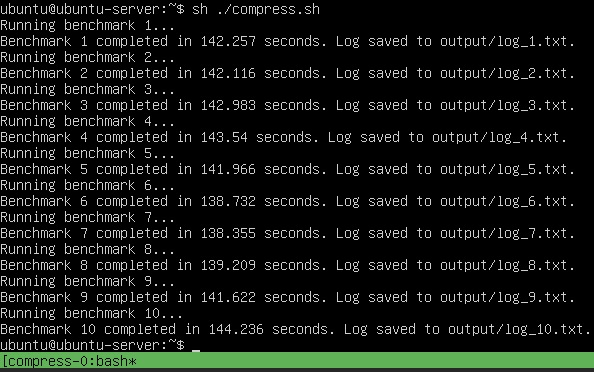
\includegraphics[width=1\textwidth]
    {assets/pics/video-compression-test/original.jpeg}
    \caption{Test Kompresi Video dengan Konfigurasi Default}
    \label{fig:video_compression_test_original}
\end{figure}

\begin{figure}
    \centering
    \begin{tikzpicture}
        \begin{axis}[
                xbar,
                bar width=12pt,
                xlabel={Detik},
                ytick=data,
                nodes near coords,
                nodes near coords align={horizontal},
                symbolic y coords={run 1,run 2,run 3,run 4,run 5,run 6,run 7,run 8,run 9,run 10},
                enlarge y limits=0.2,
                enlarge x limits=0.05,
                width=\textwidth,
                height=0.4\textheight,
                xmin=0,
                xmax=160
            ]
            \addplot [fill=black] coordinates {
                    (142.257,run 1)
                    (142.116,run 2)
                    (142.983,run 3)
                    (143.54,run 4)
                    (141.966,run 5)
                    (138.732,run 6)
                    (138.355,run 7)
                    (139.209,run 8)
                    (141.622,run 9)
                    (144.236,run 10)
                };
        \end{axis}
    \end{tikzpicture}
    \caption{Grafik Tes Kompresi Video dengan Konfigurasi Default}
    \label{fig:video_compression_test_original_graph}
\end{figure}

Program benchmark dengan kode \ref{code:kode_pengujian_kompresi_video} dijalankan pada konfigurasi default Hypervisor KVM. Hasil pengujian dapat dilihat pada gambar \ref{fig:video_compression_test_original}. Dari log yang dihasilkan saat menjalankan program benchmark, waktu yang diperlukan untuk melakukan setiap run benchmark diambil dan digunakan untuk membuat grafik seperti yang terlihat pada gambar \ref{fig:video_compression_test_original_graph}. Grafik tersebut menunjukkan bahwa waktu yang diperlukan untuk melakukan benchmark pada konfigurasi default berkisar antara 138 detik hingga 144 detik. Rata-rata dari 10 run yang dilakukan adalah 141.5 detik.

%-----------------------------------------------------------------------------%
\subsection{Konfigurasi dengan SSSE3}
%-----------------------------------------------------------------------------%
\begin{figure}
    % \centering
    % \includegraphics[width=1\textwidth]
    % {assets/pics/video-compression-test/lscpu_ssse3.jpeg}
    \texttt{fpu de pse tsc msr pae mce cx8 apic sep mtrr pge mca cmov pat pse36 clflush mmx fxsr sse sse2 ht syscall nx lm rep\_good nopl cpuid extd\_apicid tsc\_known\_freq pni \textbf{ssse3} cx16 x2apic hypervisor lahf\_lm cmp\_legacy svm 3dnowprefetch vmmcall}
    \caption{\texttt{lscpu} Konfigurasi SSSE3}
    \label{fig:lscpu_video_compression_test_ssse3}
\end{figure}

Gambar \ref{fig:lscpu_video_compression_test_ssse3} menunjukkan hasil dari perintah \texttt{lscpu} pada konfigurasi SSSE3. Konfigurasi ini memiliki perubahan flag cpu \texttt{ssse3}.

\begin{figure}
    \centering
    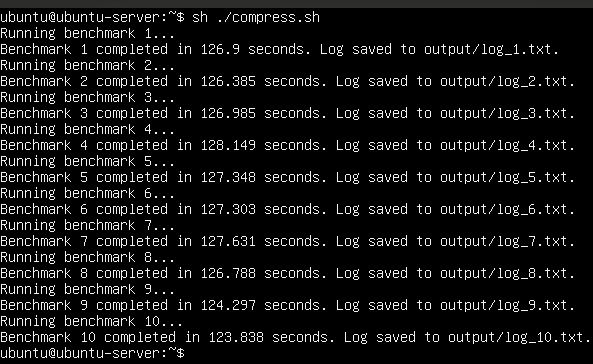
\includegraphics[width=1\textwidth]
    {assets/pics/video-compression-test/ssse3.jpeg}
    \caption{Test Kompresi Video dengan Konfigurasi SSSE3}
    \label{fig:video_compression_test_ssse3}
\end{figure}

\begin{figure}
    \centering
    \begin{tikzpicture}
        \begin{axis}[
                xbar,
                bar width=12pt,
                xlabel={Detik},
                ytick=data,
                nodes near coords,
                nodes near coords align={horizontal},
                symbolic y coords={run 1,run 2,run 3,run 4,run 5,run 6,run 7,run 8,run 9,run 10},
                enlarge y limits=0.2,
                enlarge x limits=0.05,
                width=\textwidth,
                height=0.4\textheight,
                xmin=0,
                xmax=160
            ]
            \addplot [fill=black] coordinates {
                    (126.900,run 1)
                    (126.385,run 2)
                    (126.985,run 3)
                    (128.149,run 4)
                    (127.348,run 5)
                    (127.303,run 6)
                    (127.631,run 7)
                    (126.788,run 8)
                    (124.297,run 9)
                    (123.838,run 10)
                };
        \end{axis}
    \end{tikzpicture}
    \caption{Grafik Tes Kompresi Video dengan Konfigurasi SSSE3}
    \label{fig:video_compression_test_ssse3_graph}
\end{figure}

Program benchmark dengan kode \ref{code:kode_pengujian_kompresi_video} dijalankan pada konfigurasi SSSE3. Hasil pengujian dapat dilihat pada gambar \ref{fig:video_compression_test_ssse3}. Dari log yang dihasilkan saat menjalankan program benchmark, waktu yang diperlukan untuk melakukan setiap run benchmark diambil dan digunakan untuk membuat grafik seperti yang terlihat pada gambar \ref{fig:video_compression_test_ssse3_graph}. Grafik tersebut menunjukkan bahwa waktu yang diperlukan untuk melakukan benchmark pada konfigurasi SSSE3 berkisar antara 123 detik hingga 128 detik. Rata-rata dari 10 run yang dilakukan adalah 126.5 detik.

%-----------------------------------------------------------------------------%
\subsection{Konfigurasi dengan SSE4.1}
%-----------------------------------------------------------------------------%
\begin{figure}
    % \centering
    % \includegraphics[width=1\textwidth]
    % {assets/pics/video-compression-test/lscpu_sse4.1.jpeg}
    \texttt{fpu de pse tsc msr pae mce cx8 apic sep mtrr pge mca cmov pat pse36 clflush mmx fxsr sse sse2 ht syscall nx lm rep\_good nopl cpuid extd\_apicid tsc\_known\_freq pni cx16 \textbf{sse4\_1} x2apic hypervisor lahf\_lm cmp\_legacy svm 3dnowprefetch vmmcall}
    \caption{\texttt{lscpu} Konfigurasi SSE4.1}
    \label{fig:lscpu_video_compression_test_sse4.1}
\end{figure}

Gambar \ref{fig:lscpu_video_compression_test_sse4.1} menunjukkan hasil dari perintah \texttt{lscpu} pada konfigurasi SSE4.1. Konfigurasi ini memiliki perubahan flag cpu \texttt{sse4.1}.

\begin{figure}
    \centering
    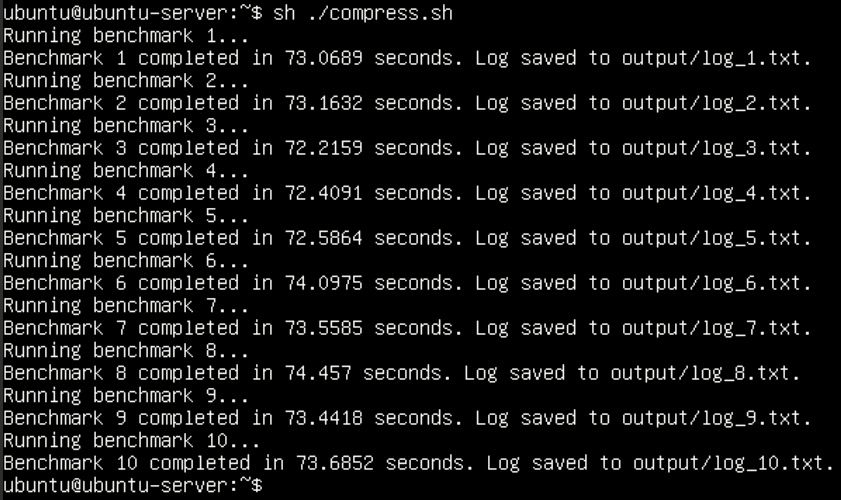
\includegraphics[width=1\textwidth]
    {assets/pics/video-compression-test/sse4.1.jpeg}
    \caption{Test Kompresi Video dengan Konfigurasi SSE4.1}
    \label{fig:video_compression_test_sse4.1}
\end{figure}

\begin{figure}
    \centering
    \begin{tikzpicture}
        \begin{axis}[
                xbar,
                bar width=12pt,
                xlabel={Detik},
                ytick=data,
                nodes near coords,
                nodes near coords align={horizontal},
                symbolic y coords={run 1,run 2,run 3,run 4,run 5,run 6,run 7,run 8,run 9,run 10},
                enlarge y limits=0.2,
                enlarge x limits=0.05,
                width=\textwidth,
                height=0.4\textheight,
                xmin=0,
                xmax=160
            ]
            \addplot [fill=black] coordinates {
                    (73.0689,run 1)
                    (73.1632,run 2)
                    (72.2159,run 3)
                    (72.4091,run 4)
                    (72.5864,run 5)
                    (74.0975,run 6)
                    (73.5585,run 7)
                    (74.4570,run 8)
                    (73.4418,run 9)
                    (73.6850,run 10)
                };
        \end{axis}
    \end{tikzpicture}
    \caption{Grafik Tes Kompresi Video dengan Konfigurasi SSE4.1}
    \label{fig:video_compression_test_sse4.1_graph}
\end{figure}

Program benchmark dengan kode \ref{code:kode_pengujian_kompresi_video} dijalankan pada konfigurasi SSE4.1. Hasil pengujian dapat dilihat pada gambar \ref{fig:video_compression_test_sse4.1}. Dari log yang dihasilkan saat menjalankan program benchmark, waktu yang diperlukan untuk melakukan setiap run benchmark diambil dan digunakan untuk membuat grafik seperti yang terlihat pada gambar \ref{fig:video_compression_test_sse4.1_graph}. Grafik tersebut menunjukkan bahwa waktu yang diperlukan untuk melakukan benchmark pada konfigurasi SSE4.1 berkisar antara 72 detik hingga 74 detik. Rata-rata dari 10 run yang dilakukan adalah 73.2 detik.

%-----------------------------------------------------------------------------%
\subsection{Konfigurasi dengan SSE4.2}
%-----------------------------------------------------------------------------%
\begin{figure}
    % \centering
    % \includegraphics[width=1\textwidth]
    % {assets/pics/video-compression-test/lscpu_sse4.2.jpeg}
    \texttt{fpu de pse tsc msr pae mce cx8 apic sep mtrr pge mca cmov pat pse36 clflush mmx fxsr sse sse2 ht syscall nx lm rep\_good nopl cpuid extd\_apicid tsc\_known\_freq pni cx16 \textbf{sse4\_2} x2apic hypervisor lahf\_lm cmp\_legacy svm 3dnowprefetch vmmcall}
    \caption{\texttt{lscpu} Konfigurasi SSE4.2}
    \label{fig:lscpu_video_compression_test_sse4.2}
\end{figure}

Gambar \ref{fig:lscpu_video_compression_test_sse4.2} menunjukkan hasil dari perintah \texttt{lscpu} pada konfigurasi SSE4.2. Konfigurasi ini memiliki perubahan flag cpu \texttt{sse4.2}.

\begin{figure}
    \centering
    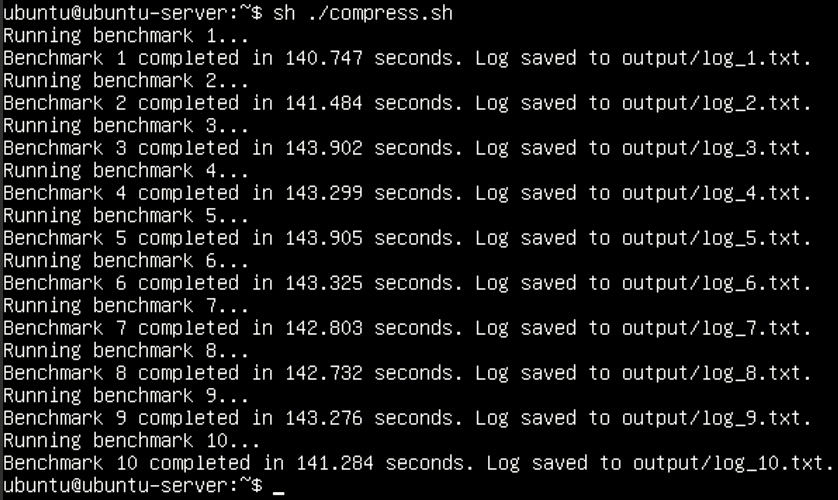
\includegraphics[width=1\textwidth]
    {assets/pics/video-compression-test/sse4.2.jpeg}
    \caption{Test Kompresi Video dengan Konfigurasi SSE4.2}
    \label{fig:video_compression_test_sse4.2}
\end{figure}

\begin{figure}
    \centering
    \begin{tikzpicture}
        \begin{axis}[
                xbar,
                bar width=12pt,
                xlabel={Detik},
                ytick=data,
                nodes near coords,
                nodes near coords align={horizontal},
                symbolic y coords={run 1,run 2,run 3,run 4,run 5,run 6,run 7,run 8,run 9,run 10},
                enlarge y limits=0.2,
                enlarge x limits=0.05,
                width=\textwidth,
                height=0.4\textheight,
                xmin=0,
                xmax=160
            ]
            \addplot [fill=black] coordinates {
                    (140.747,run 1)
                    (141.484,run 2)
                    (143.902,run 3)
                    (143.299,run 4)
                    (143.905,run 5)
                    (143.325,run 6)
                    (143.803,run 7)
                    (142.732,run 8)
                    (143.276,run 9)
                    (141.284,run 10)
                };
        \end{axis}
    \end{tikzpicture}
    \caption{Grafik Tes Kompresi Video dengan Konfigurasi SSE4.2}
    \label{fig:video_compression_test_sse4.2_graph}
\end{figure}

Program benchmark dengan kode \ref{code:kode_pengujian_kompresi_video} dijalankan pada konfigurasi SSE4.2. Hasil pengujian dapat dilihat pada gambar \ref{fig:video_compression_test_sse4.2}. Dari log yang dihasilkan saat menjalankan program benchmark, waktu yang diperlukan untuk melakukan setiap run benchmark diambil dan digunakan untuk membuat grafik seperti yang terlihat pada gambar \ref{fig:video_compression_test_sse4.2_graph}. Grafik tersebut menunjukkan bahwa waktu yang diperlukan untuk melakukan benchmark pada konfigurasi SSE4.2 berkisar antara 140 detik hingga 143 detik. Rata-rata dari 10 run yang dilakukan adalah 142.7 detik.

%-----------------------------------------------------------------------------%
\subsection{Konfigurasi dengan SSE4a}
%-----------------------------------------------------------------------------%
\begin{figure}
    % \centering
    % \includegraphics[width=1\textwidth]
    % {assets/pics/video-compression-test/lscpu_sse4a.jpeg}
    \texttt{fpu de pse tsc msr pae mce cx8 apic sep mtrr pge mca cmov pat pse36 clflush mmx fxsr sse sse2 ht syscall nx lm rep\_good nopl cpuid extd\_apicid tsc\_known\_freq pni cx16 x2apic hypervisor lahf\_lm cmp\_legacy svm \textbf{sse4a} 3dnowprefetch vmmcall}
    \caption{\texttt{lscpu} Konfigurasi SSE4a}
    \label{fig:lscpu_video_compression_test_sse4a}
\end{figure}

Gambar \ref{fig:lscpu_video_compression_test_sse4a} menunjukkan hasil dari perintah \texttt{lscpu} pada konfigurasi SSE4a. Konfigurasi ini memiliki perubahan flag cpu \texttt{sse4a}.

\begin{figure}
    \centering
    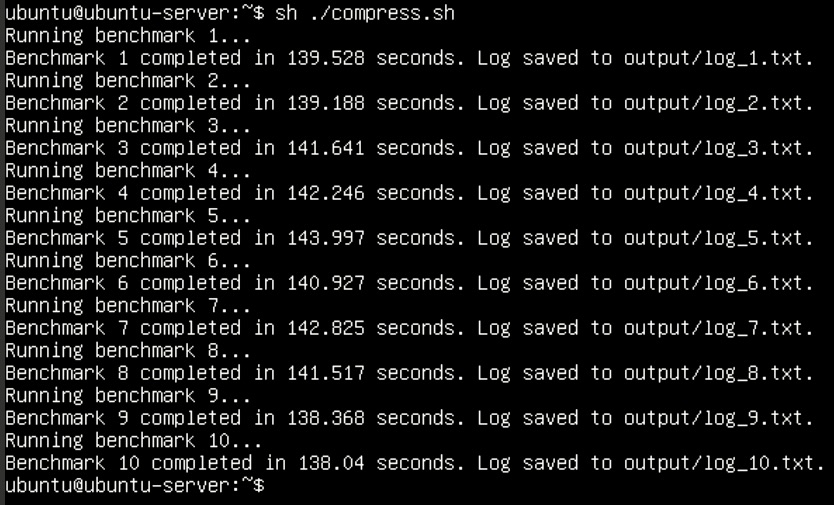
\includegraphics[width=1\textwidth]
    {assets/pics/video-compression-test/sse4a.jpeg}
    \caption{Test Kompresi Video dengan Konfigurasi SSE4a}
    \label{fig:video_compression_test_sse4a}
\end{figure}

\begin{figure}
    \centering
    \begin{tikzpicture}
        \begin{axis}[
                xbar,
                bar width=12pt,
                xlabel={Detik},
                ytick=data,
                nodes near coords,
                nodes near coords align={horizontal},
                symbolic y coords={run 1,run 2,run 3,run 4,run 5,run 6,run 7,run 8,run 9,run 10},
                enlarge y limits=0.2,
                enlarge x limits=0.05,
                width=\textwidth,
                height=0.4\textheight,
                xmin=0,
                xmax=160
            ]
            \addplot [fill=black] coordinates {
                    (139.528,run 1)
                    (139.188,run 2)
                    (141.641,run 3)
                    (142.246,run 4)
                    (143.997,run 5)
                    (140.927,run 6)
                    (142.825,run 7)
                    (141.517,run 8)
                    (138.368,run 9)
                    (138.040,run 10)
                };
        \end{axis}
    \end{tikzpicture}
    \caption{Grafik Tes Kompresi Video dengan Konfigurasi SSE4a}
    \label{fig:video_compression_test_sse4a_graph}
\end{figure}

Program benchmark dengan kode \ref{code:kode_pengujian_kompresi_video} dijalankan pada konfigurasi SSE4a. Hasil pengujian dapat dilihat pada gambar \ref{fig:video_compression_test_sse4a}. Dari log yang dihasilkan saat menjalankan program benchmark, waktu yang diperlukan untuk melakukan setiap run benchmark diambil dan digunakan untuk membuat grafik seperti yang terlihat pada gambar \ref{fig:video_compression_test_sse4a_graph}. Grafik tersebut menunjukkan bahwa waktu yang diperlukan untuk melakukan benchmark pada konfigurasi SSE4a berkisar antara 138 detik hingga 143 detik. Rata-rata dari 10 run yang dilakukan adalah 140.8 detik.
%-----------------------------------------------------------------------------%
\subsection{Konfigurasi dengan SSSE3 + SSE4.1}
%-----------------------------------------------------------------------------%
\begin{figure}
    % \centering
    % \includegraphics[width=1\textwidth]
    % {assets/pics/video-compression-test/lscpu_ssse3,sse4.1.jpeg}
    \texttt{fpu de pse tsc msr pae mce cx8 apic sep mtrr pge mca cmov pat pse36 clflush mmx fxsr sse sse2 ht syscall nx lm rep\_good nopl cpuid extd\_apicid tsc\_known\_freq pni \textbf{ssse3} cx16 \textbf{sse4\_1} x2apic hypervisor lahf\_lm cmp\_legacy svm 3dnowprefetch vmmcall}
    \caption{\texttt{lscpu} Konfigurasi SSSE3 + SSE4.1}
    \label{fig:lscpu_video_compression_test_ssse3,sse4.1}
\end{figure}

Gambar \ref{fig:lscpu_video_compression_test_ssse3,sse4.1} menunjukkan hasil dari perintah \texttt{lscpu} pada konfigurasi SSSE3 + SSE4.1. Konfigurasi ini memiliki perubahan flag cpu \texttt{ssse3} dan \texttt{sse4.1}.

\begin{figure}
    \centering
    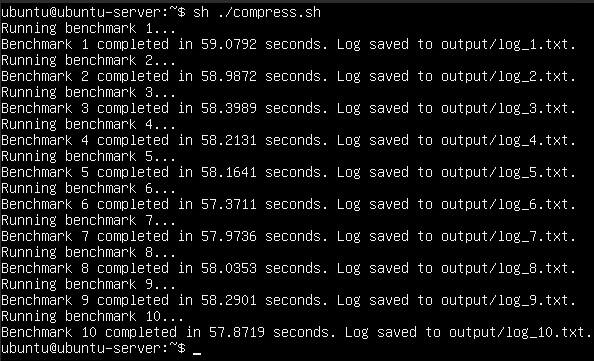
\includegraphics[width=1\textwidth]
    {assets/pics/video-compression-test/ssse3,sse4.1.jpeg}
    \caption{Test Kompresi Video dengan Konfigurasi SSSE3 + SSE4.1}
    \label{fig:video_compression_test_ssse3,sse4.1}
\end{figure}

\begin{figure}
    \centering
    \begin{tikzpicture}
        \begin{axis}[
                xbar,
                bar width=12pt,
                xlabel={Detik},
                ytick=data,
                nodes near coords,
                nodes near coords align={horizontal},
                symbolic y coords={run 1,run 2,run 3,run 4,run 5,run 6,run 7,run 8,run 9,run 10},
                enlarge y limits=0.2,
                enlarge x limits=0.05,
                width=\textwidth,
                height=0.4\textheight,
                xmin=0,
                xmax=160
            ]
            \addplot [fill=black] coordinates {
                    (59.079,run 1)
                    (58.987,run 2)
                    (58.396,run 3)
                    (58.213,run 4)
                    (58.164,run 5)
                    (57.371,run 6)
                    (57.973,run 7)
                    (58.035,run 8)
                    (58.290,run 9)
                    (57.871,run 10)
                };
        \end{axis}
    \end{tikzpicture}
    \caption{Grafik Tes Kompresi Video dengan Konfigurasi SSSE3 + SSE4.1}
    \label{fig:video_compression_test_ssse3,sse4.1_graph}
\end{figure}

Program benchmark dengan kode \ref{code:kode_pengujian_kompresi_video} dijalankan pada konfigurasi SSSE3 + SSE4.1. Hasil pengujian dapat dilihat pada gambar \ref{fig:video_compression_test_ssse3,sse4.1}. Dari log yang dihasilkan saat menjalankan program benchmark, waktu yang diperlukan untuk melakukan setiap run benchmark diambil dan digunakan untuk membuat grafik seperti yang terlihat pada gambar \ref{fig:video_compression_test_ssse3,sse4.1_graph}. Grafik tersebut menunjukkan bahwa waktu yang diperlukan untuk melakukan benchmark pada konfigurasi SSSE3 + SSE4.1 berkisar antara 57 detik hingga 59 detik. Rata-rata dari 10 run yang dilakukan adalah 58.2 detik.

%-----------------------------------------------------------------------------%
\subsection{Konfigurasi dengan SSSE3 + SSE4.2}
%-----------------------------------------------------------------------------%
\begin{figure}
    % \centering
    % \includegraphics[width=1\textwidth]
    % {assets/pics/video-compression-test/lscpu_ssse3,sse4.2.jpeg}
    \texttt{fpu de pse tsc msr pae mce cx8 apic sep mtrr pge mca cmov pat pse36 clflush mmx fxsr sse sse2 ht syscall nx lm rep\_good nopl cpuid extd\_apicid tsc\_known\_freq pni \textbf{ssse3} cx16 \textbf{sse4\_2} x2apic hypervisor lahf\_lm cmp\_legacy svm 3dnowprefetch vmmcall}
    \caption{\texttt{lscpu} Konfigurasi SSSE3 + SSE4.2}
    \label{fig:lscpu_video_compression_test_ssse3,sse4.2}
\end{figure}

Gambar \ref{fig:lscpu_video_compression_test_ssse3,sse4.2} menunjukkan hasil dari perintah \texttt{lscpu} pada konfigurasi SSSE3 + SSE4.2. Konfigurasi ini memiliki perubahan flag cpu \texttt{ssse3} dan \texttt{sse4.2}.

\begin{figure}
    \centering
    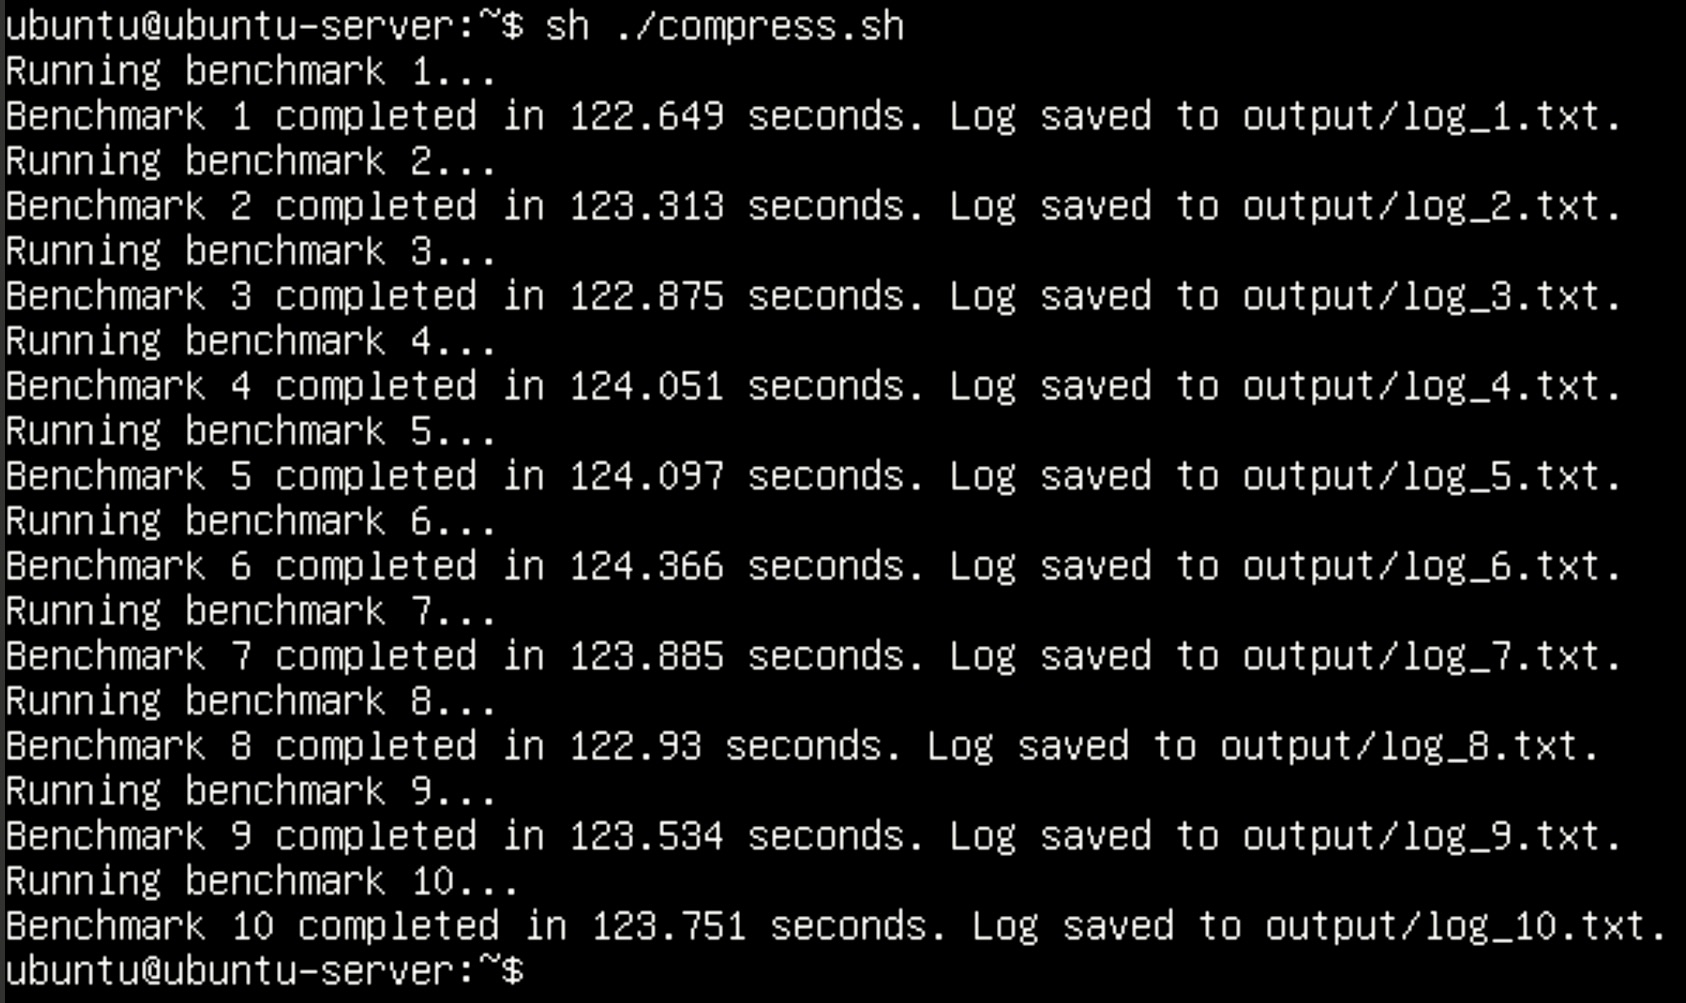
\includegraphics[width=1\textwidth]
    {assets/pics/video-compression-test/ssse3,sse4.2.jpeg}
    \caption{Test Kompresi Video dengan Konfigurasi SSSE3 + SSE4.2}
    \label{fig:video_compression_test_ssse3,sse4.2}
\end{figure}

\begin{figure}
    \centering
    \begin{tikzpicture}
        \begin{axis}[
                xbar,
                bar width=12pt,
                xlabel={Detik},
                ytick=data,
                nodes near coords,
                nodes near coords align={horizontal},
                symbolic y coords={run 1,run 2,run 3,run 4,run 5,run 6,run 7,run 8,run 9,run 10},
                enlarge y limits=0.2,
                enlarge x limits=0.05,
                width=\textwidth,
                height=0.4\textheight,
                xmin=0,
                xmax=160
            ]
            \addplot [fill=black] coordinates {
                    (122.649,run 1)
                    (123.313,run 2)
                    (122.875,run 3)
                    (124.051,run 4)
                    (124.097,run 5)
                    (124.366,run 6)
                    (123.885,run 7)
                    (122.930,run 8)
                    (123.534,run 9)
                    (123.751,run 10)
                };
        \end{axis}
    \end{tikzpicture}
    \caption{Grafik Tes Kompresi Video dengan Konfigurasi SSSE3 + SSE4.2}
    \label{fig:video_compression_test_ssse3,sse4.2_graph}
\end{figure}

Program benchmark dengan kode \ref{code:kode_pengujian_kompresi_video} dijalankan pada konfigurasi SSSE3 + SSE4.2. Hasil pengujian dapat dilihat pada gambar \ref{fig:video_compression_test_ssse3,sse4.2}. Dari log yang dihasilkan saat menjalankan program benchmark, waktu yang diperlukan untuk melakukan setiap run benchmark diambil dan digunakan untuk membuat grafik seperti yang terlihat pada gambar \ref{fig:video_compression_test_ssse3,sse4.2_graph}. Grafik tersebut menunjukkan bahwa waktu yang diperlukan untuk melakukan benchmark pada konfigurasi SSSE3 + SSE4.2 berkisar antara 122 detik hingga 124 detik. Rata-rata dari 10 run yang dilakukan adalah 123.5 detik.

%-----------------------------------------------------------------------------%
\subsection{Konfigurasi dengan SSSE3 + SSE4a}
%-----------------------------------------------------------------------------%
\begin{figure}
    % \centering
    % \includegraphics[width=1\textwidth]
    % {assets/pics/video-compression-test/lscpu_ssse3,sse4a.jpeg}
    \texttt{fpu de pse tsc msr pae mce cx8 apic sep mtrr pge mca cmov pat pse36 clflush mmx fxsr sse sse2 ht syscall nx lm rep\_good nopl cpuid extd\_apicid tsc\_known\_freq pni \textbf{ssse3} cx16 x2apic hypervisor lahf\_lm cmp\_legacy svm \textbf{sse4a} 3dnowprefetch vmmcall}
    \caption{\texttt{lscpu} Konfigurasi SSSE3 + SSE4a}
    \label{fig:lscpu_video_compression_test_ssse3,sse4a}
\end{figure}

Gambar \ref{fig:lscpu_video_compression_test_ssse3,sse4a} menunjukkan hasil dari perintah \texttt{lscpu} pada konfigurasi SSSE3 + SSE4a. Konfigurasi ini memiliki perubahan flag cpu \texttt{ssse3} dan \texttt{sse4a}.

\begin{figure}
    \centering
    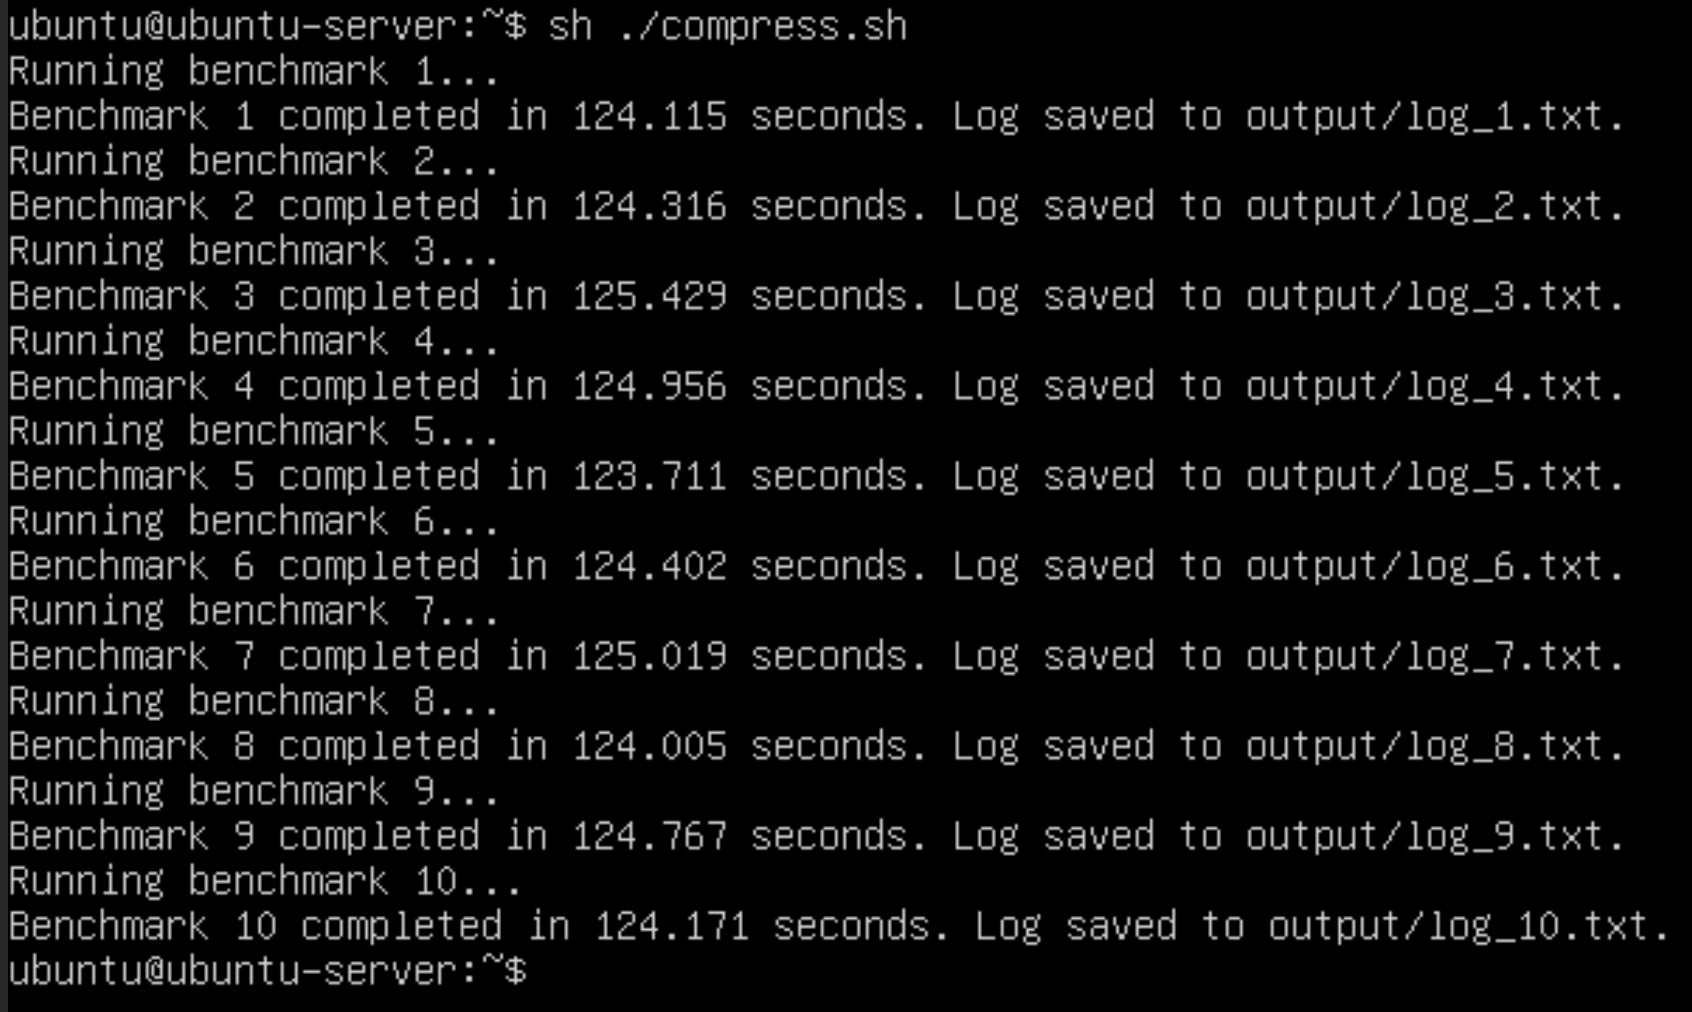
\includegraphics[width=1\textwidth]
    {assets/pics/video-compression-test/ssse3,sse4a.jpeg}
    \caption{Test Kompresi Video dengan Konfigurasi SSSE3 + SSE4a}
    \label{fig:video_compression_test_ssse3,sse4a}
\end{figure}

\begin{figure}
    \centering
    \begin{tikzpicture}
        \begin{axis}[
                xbar,
                bar width=12pt,
                xlabel={Detik},
                ytick=data,
                nodes near coords,
                nodes near coords align={horizontal},
                symbolic y coords={run 1,run 2,run 3,run 4,run 5,run 6,run 7,run 8,run 9,run 10},
                enlarge y limits=0.2,
                enlarge x limits=0.05,
                width=\textwidth,
                height=0.4\textheight,
                xmin=0,
                xmax=160
            ]
            \addplot [fill=black] coordinates {
                    (124.115,run 1)
                    (124.316,run 2)
                    (125.429,run 3)
                    (124.956,run 4)
                    (123.711,run 5)
                    (124.402,run 6)
                    (125.019,run 7)
                    (124.005,run 8)
                    (124.767,run 9)
                    (124.171,run 10)
                };
        \end{axis}
    \end{tikzpicture}
    \caption{Grafik Tes Kompresi Video dengan Konfigurasi SSSE3 + SSE4a}
    \label{fig:video_compression_test_ssse3,sse4a_graph}
\end{figure}

Program benchmark dengan kode \ref{code:kode_pengujian_kompresi_video} dijalankan pada konfigurasi SSSE3 + SSE4a. Hasil pengujian dapat dilihat pada gambar \ref{fig:video_compression_test_ssse3,sse4a}. Dari log yang dihasilkan saat menjalankan program benchmark, waktu yang diperlukan untuk melakukan setiap run benchmark diambil dan digunakan untuk membuat grafik seperti yang terlihat pada gambar \ref{fig:video_compression_test_ssse3,sse4a_graph}. Grafik tersebut menunjukkan bahwa waktu yang diperlukan untuk melakukan benchmark pada konfigurasi SSSE3 + SSE4a berkisar antara 123 detik hingga 125 detik. Rata-rata dari 10 run yang dilakukan adalah 124.4 detik.

%-----------------------------------------------------------------------------%
\subsection{Konfigurasi dengan SSE4.1 + SSE4.2}
%-----------------------------------------------------------------------------%
\begin{figure}
    % \centering
    % \includegraphics[width=1\textwidth]
    % {assets/pics/video-compression-test/lscpu_sse4.1,sse4.2.jpeg}
    \texttt{fpu de pse tsc msr pae mce cx8 apic sep mtrr pge mca cmov pat pse36 clflush mmx fxsr sse sse2 ht syscall nx lm rep\_good nopl cpuid extd\_apicid tsc\_known\_freq pni cx16 \textbf{sse4\_1} \textbf{sse4\_2} x2apic hypervisor lahf\_lm cmp\_legacy svm 3dnowprefetch vmmcall}
    \caption{\texttt{lscpu} Konfigurasi SSE4.1 + SSE4.2}
    \label{fig:lscpu_video_compression_test_sse4.1,sse4.2}
\end{figure}

Gambar \ref{fig:lscpu_video_compression_test_sse4.1,sse4.2} menunjukkan hasil dari perintah \texttt{lscpu} pada konfigurasi SSE4.1 + SSE4.2. Konfigurasi ini memiliki perubahan flag cpu \texttt{sse4.1} dan \texttt{sse4.2}.

\begin{figure}
    \centering
    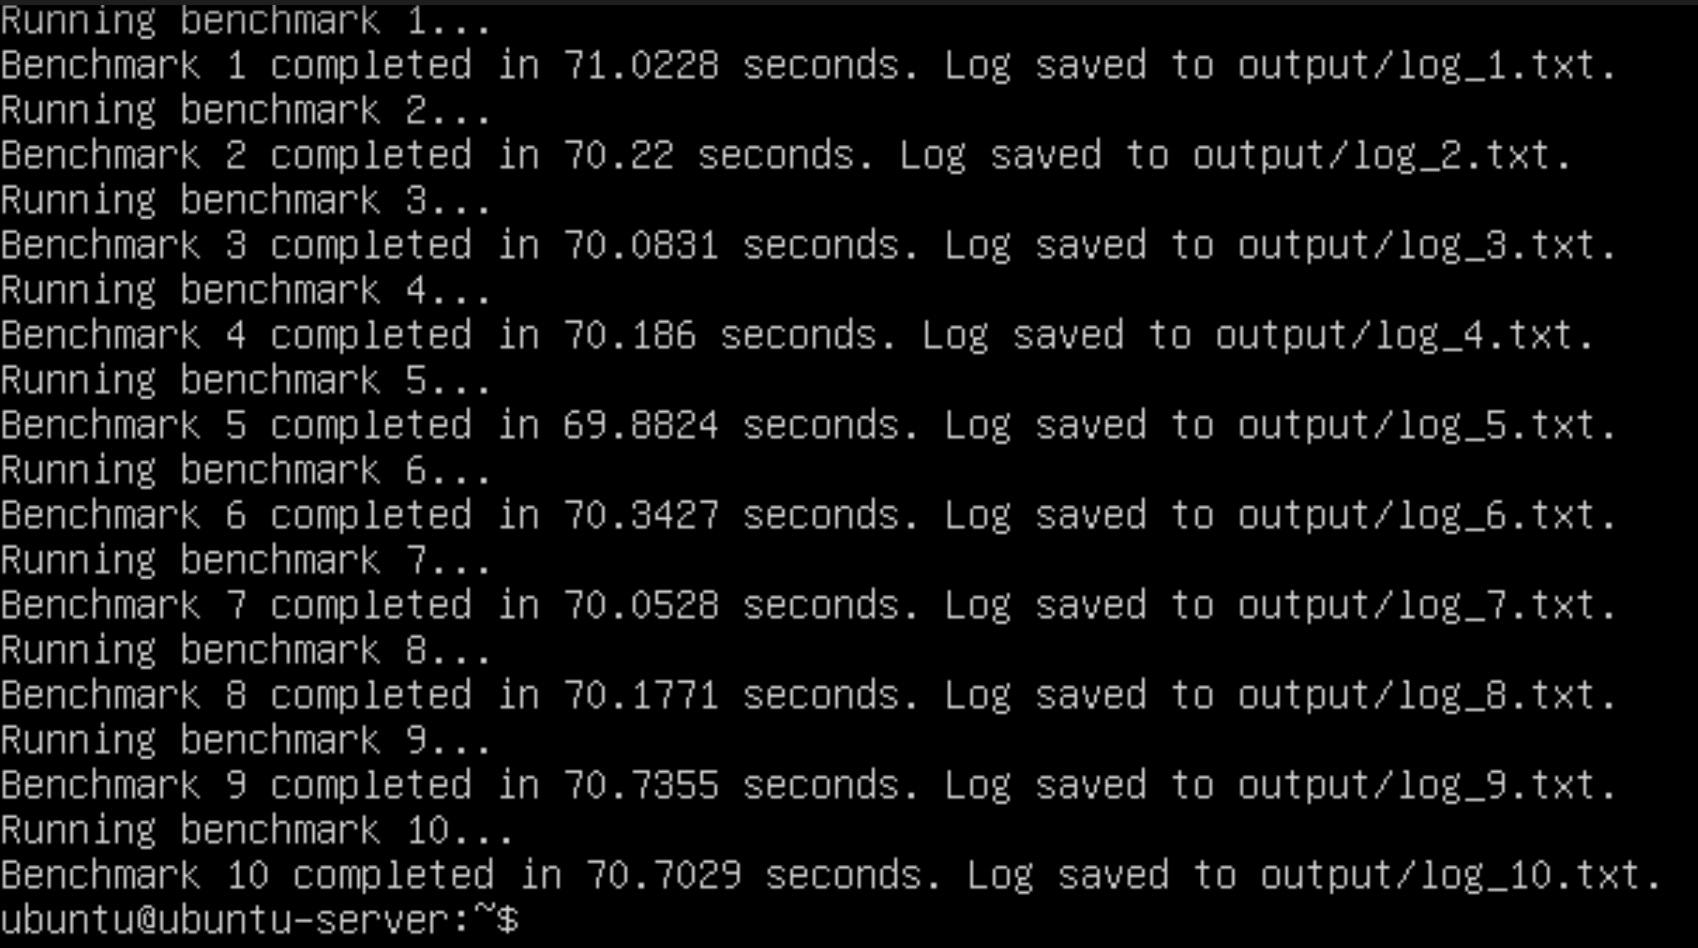
\includegraphics[width=1\textwidth]
    {assets/pics/video-compression-test/sse4.1,sse4.2.jpeg}
    \caption{Test Kompresi Video dengan Konfigurasi SSE4.1 + SSE4.2}
    \label{fig:video_compression_test_sse4.1,sse4.2}
\end{figure}

\begin{figure}
    \centering
    \begin{tikzpicture}
        \begin{axis}[
                xbar,
                bar width=12pt,
                xlabel={Detik},
                ytick=data,
                nodes near coords,
                nodes near coords align={horizontal},
                symbolic y coords={run 1,run 2,run 3,run 4,run 5,run 6,run 7,run 8,run 9,run 10},
                enlarge y limits=0.2,
                enlarge x limits=0.05,
                width=\textwidth,
                height=0.4\textheight,
                xmin=0,
                xmax=160
            ]
            \addplot [fill=black] coordinates {
                    (71.0288,run 1)
                    (70.2200,run 2)
                    (70.0831,run 3)
                    (70.1860,run 4)
                    (69.8824,run 5)
                    (70.3427,run 6)
                    (70.0528,run 7)
                    (70.1771,run 8)
                    (70.7355,run 9)
                    (70.7029,run 10)
                };
        \end{axis}
    \end{tikzpicture}
    \caption{Grafik Tes Kompresi Video dengan Konfigurasi SSE4.1 + SSE4.2}
    \label{fig:video_compression_test_sse4.1,sse4.2_graph}
\end{figure}

Program benchmark dengan kode \ref{code:kode_pengujian_kompresi_video} dijalankan pada konfigurasi SSE4.1 + SSE4.2. Hasil pengujian dapat dilihat pada gambar \ref{fig:video_compression_test_sse4.1,sse4.2}. Dari log yang dihasilkan saat menjalankan program benchmark, waktu yang diperlukan untuk melakukan setiap run benchmark diambil dan digunakan untuk membuat grafik seperti yang terlihat pada gambar \ref{fig:video_compression_test_sse4.1,sse4.2_graph}. Grafik tersebut menunjukkan bahwa waktu yang diperlukan untuk melakukan benchmark pada konfigurasi SSE4.1 + SSE4.2 berkisar antara 69 detik hingga 71 detik. Rata-rata dari 10 run yang dilakukan adalah 70.34 detik.

%-----------------------------------------------------------------------------%
\subsection{Konfigurasi dengan SSE4.1 + SSE4a}
%-----------------------------------------------------------------------------%
\begin{figure}
    % \centering
    % \includegraphics[width=1\textwidth]
    % {assets/pics/video-compression-test/lscpu_sse4.1,sse4a.jpeg}
    \texttt{fpu de pse tsc msr pae mce cx8 apic sep mtrr pge mca cmov pat pse36 clflush mmx fxsr sse sse2 ht syscall nx lm rep\_good nopl cpuid extd\_apicid tsc\_known\_freq pni cx16 \textbf{sse4\_1} x2apic hypervisor lahf\_lm cmp\_legacy svm \textbf{sse4a} 3dnowprefetch vmmcall}
    \caption{\texttt{lscpu} Konfigurasi SSE4.1 + SSE4a}
    \label{fig:lscpu_video_compression_test_sse4.1,sse4a}
\end{figure}

Gambar \ref{fig:lscpu_video_compression_test_sse4.1,sse4a} menunjukkan hasil dari perintah \texttt{lscpu} pada konfigurasi SSE4.1 + SSE4a. Konfigurasi ini memiliki perubahan flag cpu \texttt{sse4.1} dan \texttt{sse4a}.

\begin{figure}
    \centering
    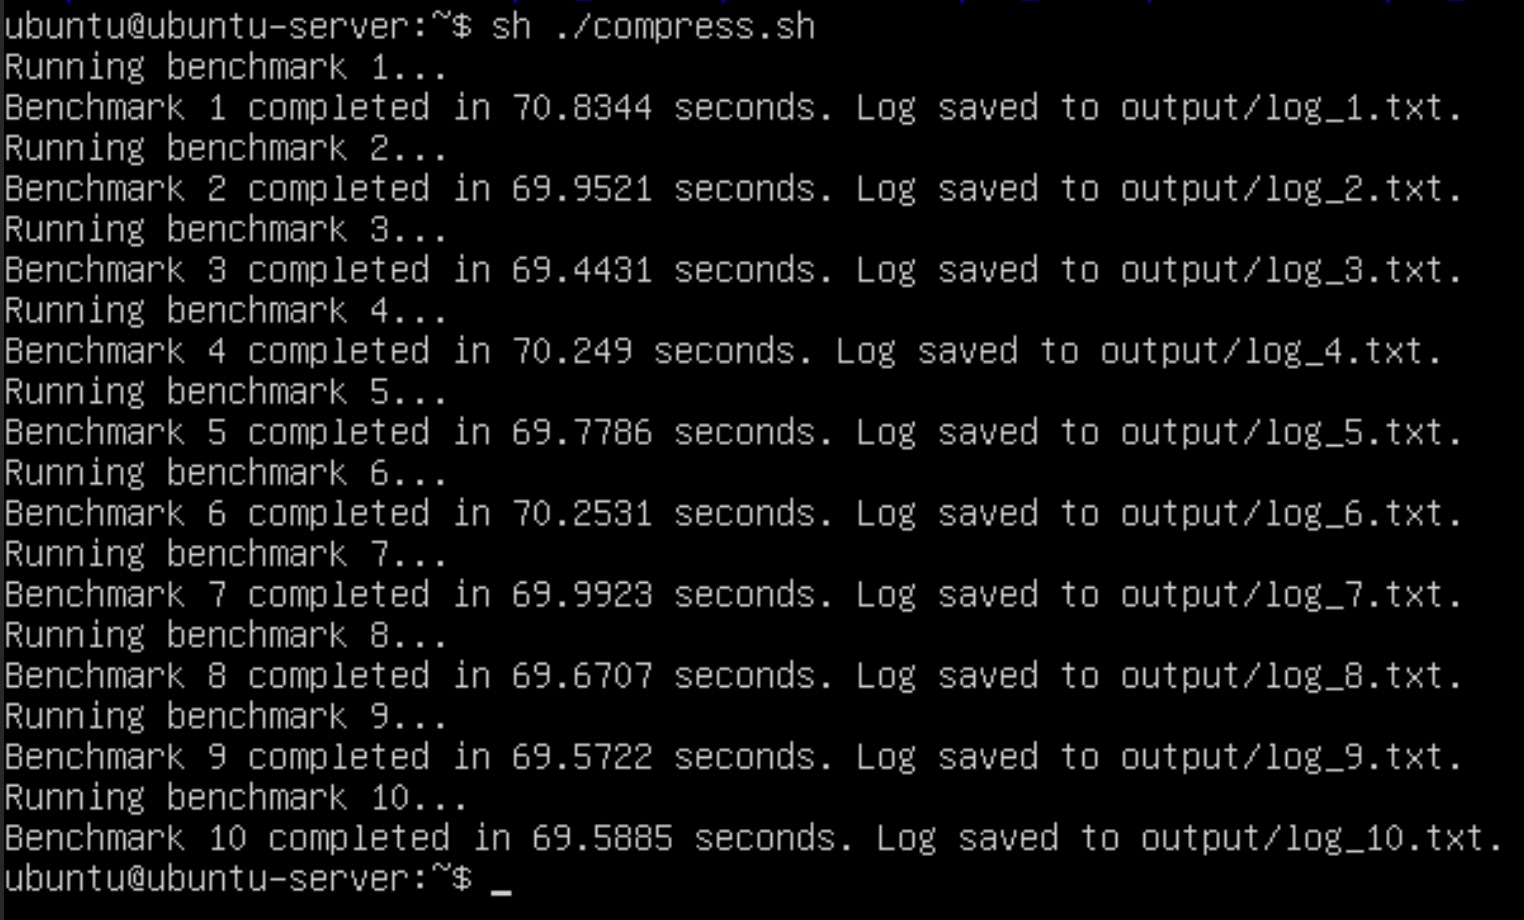
\includegraphics[width=1\textwidth]
    {assets/pics/video-compression-test/sse4.1,sse4a.jpeg}
    \caption{Test Kompresi Video dengan Konfigurasi SSE4.1 + SSE4a}
    \label{fig:video_compression_test_sse4.1,sse4a}
\end{figure}

\begin{figure}
    \centering
    \begin{tikzpicture}
        \begin{axis}[
                xbar,
                bar width=12pt,
                xlabel={Detik},
                ytick=data,
                nodes near coords,
                nodes near coords align={horizontal},
                symbolic y coords={run 1,run 2,run 3,run 4,run 5,run 6,run 7,run 8,run 9,run 10},
                enlarge y limits=0.2,
                enlarge x limits=0.05,
                width=\textwidth,
                height=0.4\textheight,
                xmin=0,
                xmax=160
            ]
            \addplot [fill=black] coordinates {
                    (70.8344,run 1)
                    (69.9521,run 2)
                    (69.4431,run 3)
                    (70.2490,run 4)
                    (69.7786,run 5)
                    (70.2531,run 6)
                    (69.9923,run 7)
                    (69.6707,run 8)
                    (69.5722,run 9)
                    (69.5885,run 10)
                };
        \end{axis}
    \end{tikzpicture}
    \caption{Grafik Tes Kompresi Video dengan Konfigurasi SSE4.1 + SSE4a}
    \label{fig:video_compression_test_sse4.1,sse4a_graph}
\end{figure}

Program benchmark dengan kode \ref{code:kode_pengujian_kompresi_video} dijalankan pada konfigurasi SSE4.1 + SSE4a. Hasil pengujian dapat dilihat pada gambar \ref{fig:video_compression_test_sse4.1,sse4a}. Dari log yang dihasilkan saat menjalankan program benchmark, waktu yang diperlukan untuk melakukan setiap run benchmark diambil dan digunakan untuk membuat grafik seperti yang terlihat pada gambar \ref{fig:video_compression_test_sse4.1,sse4a_graph}. Grafik tersebut menunjukkan bahwa waktu yang diperlukan untuk melakukan benchmark pada konfigurasi SSE4.1 + SSE4a berkisar antara 69 detik hingga 70 detik. Rata-rata dari 10 run yang dilakukan adalah 69.9 detik.

%-----------------------------------------------------------------------------%
\subsection{Konfigurasi dengan SSE4.2 + SSE4a}
%-----------------------------------------------------------------------------%
\begin{figure}
    % \centering
    % \includegraphics[width=1\textwidth]
    % {assets/pics/video-compression-test/lscpu_sse4.2,sse4a.jpeg}
    \texttt{fpu de pse tsc msr pae mce cx8 apic sep mtrr pge mca cmov pat pse36 clflush mmx fxsr sse sse2 ht syscall nx lm rep\_good nopl cpuid extd\_apicid tsc\_known\_freq pni cx16 \textbf{sse4\_2} x2apic hypervisor lahf\_lm cmp\_legacy svm \textbf{sse4a} 3dnowprefetch vmmcall}
    \caption{\texttt{lscpu} Konfigurasi SSE4.2 + SSE4a}
    \label{fig:lscpu_video_compression_test_sse4.2,sse4a}
\end{figure}

Gambar \ref{fig:lscpu_video_compression_test_sse4.2,sse4a} menunjukkan hasil dari perintah \texttt{lscpu} pada konfigurasi SSE4.2 + SSE4a. Konfigurasi ini memiliki perubahan flag cpu \texttt{sse4.2} dan \texttt{sse4a}.

\begin{figure}
    \centering
    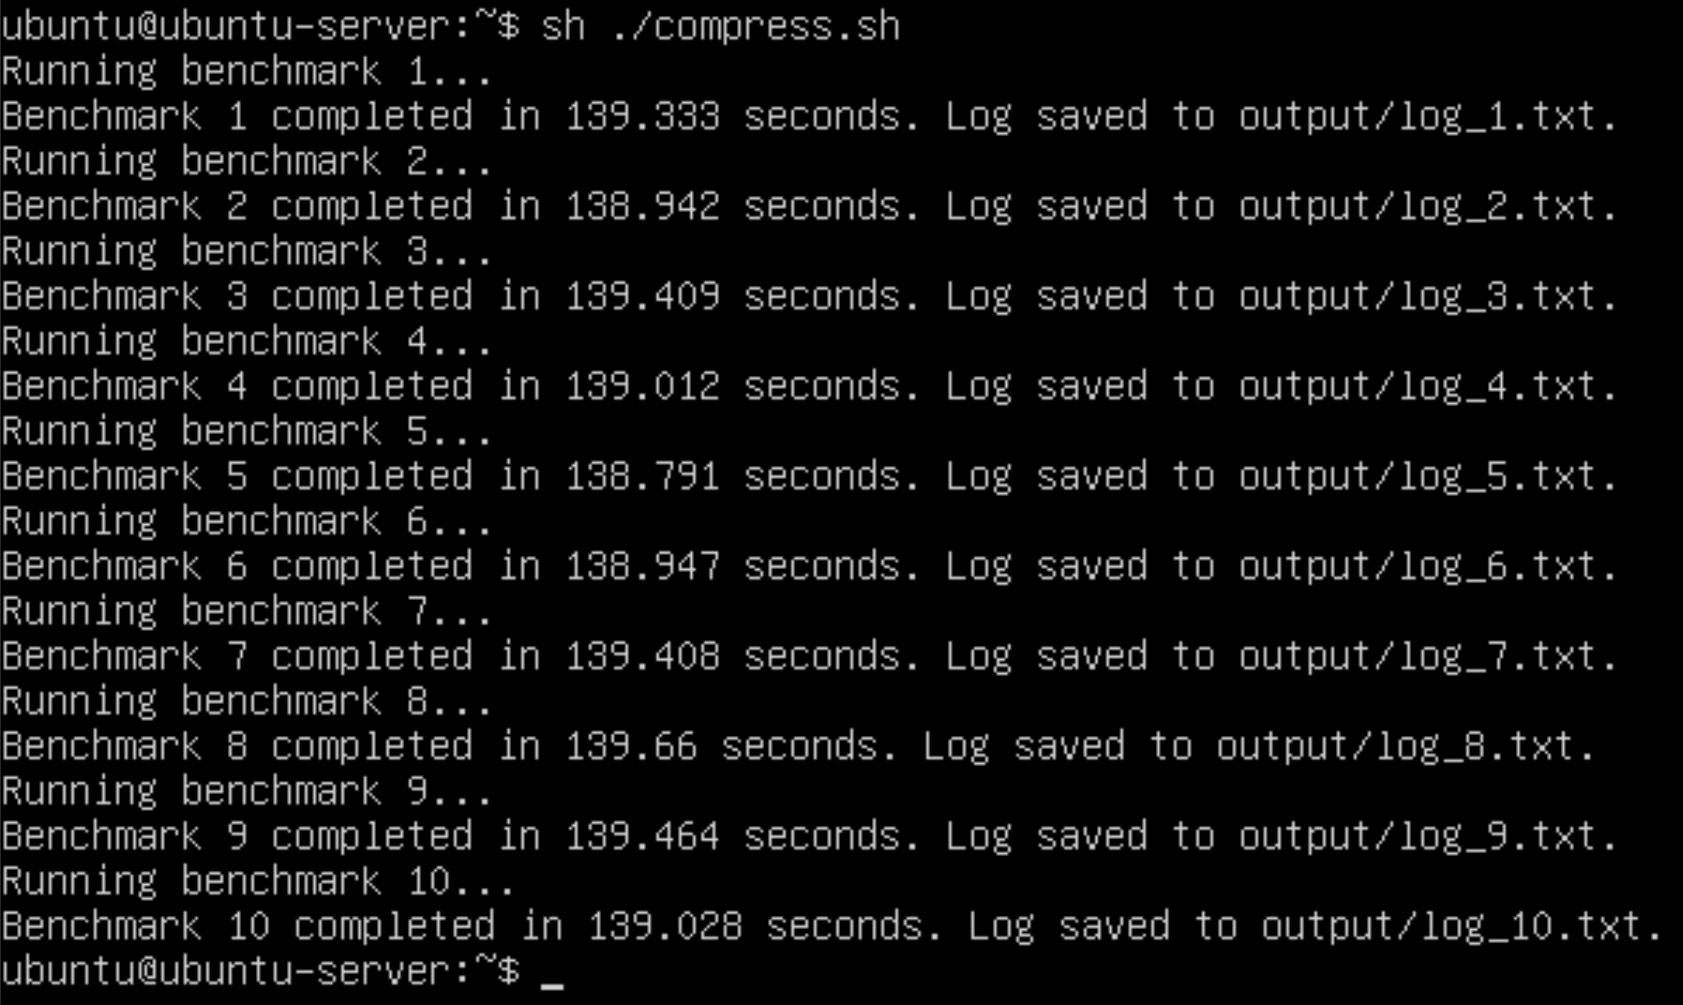
\includegraphics[width=1\textwidth]
    {assets/pics/video-compression-test/sse4.2,sse4a.jpeg}
    \caption{Test Kompresi Video dengan Konfigurasi SSE4.2 + SSE4a}
    \label{fig:video_compression_test_sse4.2,sse4a}
\end{figure}

\begin{figure}
    \centering
    \begin{tikzpicture}
        \begin{axis}[
                xbar,
                bar width=12pt,
                xlabel={Detik},
                ytick=data,
                nodes near coords,
                nodes near coords align={horizontal},
                symbolic y coords={run 1,run 2,run 3,run 4,run 5,run 6,run 7,run 8,run 9,run 10},
                enlarge y limits=0.2,
                enlarge x limits=0.05,
                width=\textwidth,
                height=0.4\textheight,
                xmin=0,
                xmax=160
            ]
            \addplot [fill=black] coordinates {
                    (139.333,run 1)
                    (138.942,run 2)
                    (139.409,run 3)
                    (139.012,run 4)
                    (138.791,run 5)
                    (138.947,run 6)
                    (139.408,run 7)
                    (139.660,run 8)
                    (139.464,run 9)
                    (139.028,run 10)
                };
        \end{axis}
    \end{tikzpicture}
    \caption{Grafik Tes Kompresi Video dengan Konfigurasi SSE4.2 + SSE4a}
    \label{fig:video_compression_test_sse4.2,sse4a_graph}
\end{figure}

Program benchmark dengan kode \ref{code:kode_pengujian_kompresi_video} dijalankan pada konfigurasi SSE4.2 + SSE4a. Hasil pengujian dapat dilihat pada gambar \ref{fig:video_compression_test_sse4.2,sse4a}. Dari log yang dihasilkan saat menjalankan program benchmark, waktu yang diperlukan untuk melakukan setiap run benchmark diambil dan digunakan untuk membuat grafik seperti yang terlihat pada gambar \ref{fig:video_compression_test_sse4.2,sse4a_graph}. Grafik tersebut menunjukkan bahwa waktu yang diperlukan untuk melakukan benchmark pada konfigurasi SSE4.2 + SSE4a berkisar antara 138 detik hingga 139 detik. Rata-rata dari 10 run yang dilakukan adalah 139.1 detik.

%-----------------------------------------------------------------------------%
\subsection{Konfigurasi dengan SSSE3 + SSE4.1 + SSE4.2}
%-----------------------------------------------------------------------------%
\begin{figure}
    % \centering
    % \includegraphics[width=1\textwidth]
    % {assets/pics/video-compression-test/lscpu_ssse3,sse4.1,sse4.2.jpeg}
    \texttt{fpu de pse tsc msr pae mce cx8 apic sep mtrr pge mca cmov pat pse36 clflush mmx fxsr sse sse2 ht syscall nx lm rep\_good nopl cpuid extd\_apicid tsc\_known\_freq pni \textbf{ssse3} cx16 \textbf{sse4\_1} \textbf{sse4\_2} x2apic hypervisor lahf\_lm cmp\_legacy svm 3dnowprefetch vmmcall}
    \caption{\texttt{lscpu} Konfigurasi SSSE3 + SSE4.1 + SSE4.2}
    \label{fig:lscpu_video_compression_test_ssse3,sse4.1,sse4.2}
\end{figure}

Gambar \ref{fig:lscpu_video_compression_test_ssse3,sse4.1,sse4.2} menunjukkan hasil dari perintah \texttt{lscpu} pada konfigurasi SSSE3 + SSE4.1 + SSE4.2. Konfigurasi ini memiliki perubahan flag cpu \texttt{ssse3}, \texttt{sse4.1}, dan \texttt{sse4.2}.

\begin{figure}
    \centering
    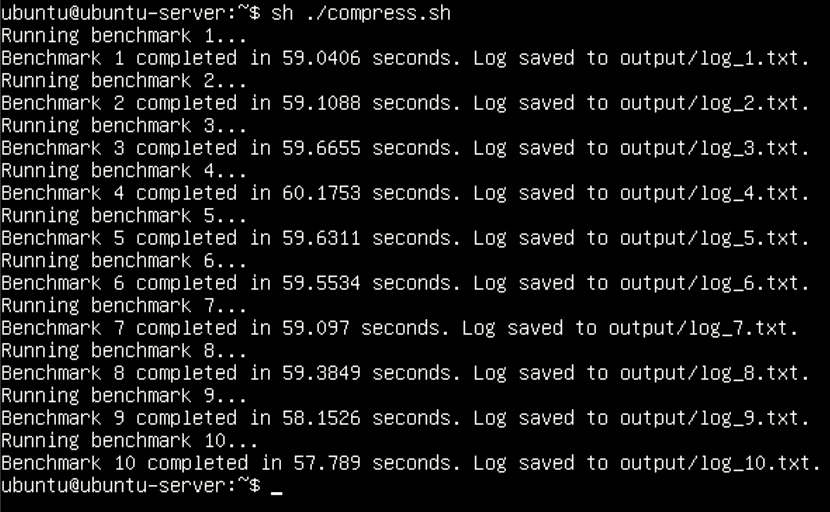
\includegraphics[width=1\textwidth]
    {assets/pics/video-compression-test/ssse3,sse4.1,sse4.2.jpeg}
    \caption{Test Kompresi Video dengan Konfigurasi SSSE3 + SSE4.1 + SSE4.2}
    \label{fig:video_compression_test_ssse3,sse4.1,sse4.2}
\end{figure}

\begin{figure}
    \centering
    \begin{tikzpicture}
        \begin{axis}[
                xbar,
                bar width=12pt,
                xlabel={Detik},
                ytick=data,
                nodes near coords,
                nodes near coords align={horizontal},
                symbolic y coords={run 1,run 2,run 3,run 4,run 5,run 6,run 7,run 8,run 9,run 10},
                enlarge y limits=0.2,
                enlarge x limits=0.05,
                width=\textwidth,
                height=0.4\textheight,
                xmin=0,
                xmax=160
            ]
            \addplot [fill=black] coordinates {
                    (59.0406,run 1)
                    (59.1088,run 2)
                    (59.6655,run 3)
                    (60.1753,run 4)
                    (59.5311,run 5)
                    (59.5534,run 6)
                    (59.0970,run 7)
                    (59.3849,run 8)
                    (58.1562,run 9)
                    (57.7890,run 10)
                };
        \end{axis}
    \end{tikzpicture}
    \caption{Grafik Tes Kompresi Video dengan Konfigurasi SSSE3 + SSE4.1 + SSE4.2}
    \label{fig:video_compression_test_ssse3,sse4.1,sse4.2_graph}
\end{figure}

Program benchmark dengan kode \ref{code:kode_pengujian_kompresi_video} dijalankan pada konfigurasi SSSE3 + SSE4.1 + SSE4.2. Hasil pengujian dapat dilihat pada gambar \ref{fig:video_compression_test_ssse3,sse4.1,sse4.2}. Dari log yang dihasilkan saat menjalankan program benchmark, waktu yang diperlukan untuk melakukan setiap run benchmark diambil dan digunakan untuk membuat grafik seperti yang terlihat pada gambar \ref{fig:video_compression_test_ssse3,sse4.1,sse4.2_graph}. Grafik tersebut menunjukkan bahwa waktu yang diperlukan untuk melakukan benchmark pada konfigurasi SSSE3 + SSE4.1 + SSE4.2 berkisar antara 57 detik hingga 60 detik. Rata-rata dari 10 run yang dilakukan adalah 59.1 detik.

%-----------------------------------------------------------------------------%
\subsection{Konfigurasi dengan SSSE3 + SSE4.1 + SSE4a}
%-----------------------------------------------------------------------------%
\begin{figure}
    % \centering
    % \includegraphics[width=1\textwidth]
    % {assets/pics/video-compression-test/lscpu_ssse3,sse4.1,sse4a.jpeg}
    \texttt{fpu de pse tsc msr pae mce cx8 apic sep mtrr pge mca cmov pat pse36 clflush mmx fxsr sse sse2 ht syscall nx lm rep\_good nopl cpuid extd\_apicid tsc\_known\_freq pni \textbf{ssse3} cx16 \textbf{sse4\_1} x2apic hypervisor lahf\_lm cmp\_legacy svm \textbf{sse4a} 3dnowprefetch vmmcall}
    \caption{\texttt{lscpu} Konfigurasi SSSE3 + SSE4.1 + SSE4a}
    \label{fig:lscpu_video_compression_test_ssse3,sse4.1,sse4a}
\end{figure}

Gambar \ref{fig:lscpu_video_compression_test_ssse3,sse4.1,sse4a} menunjukkan hasil dari perintah \texttt{lscpu} pada konfigurasi SSSE3 + SSE4.1 + SSE4a. Konfigurasi ini memiliki perubahan flag cpu \texttt{ssse3}, \texttt{sse4.1}, dan \texttt{sse4a}.

\begin{figure}
    \centering
    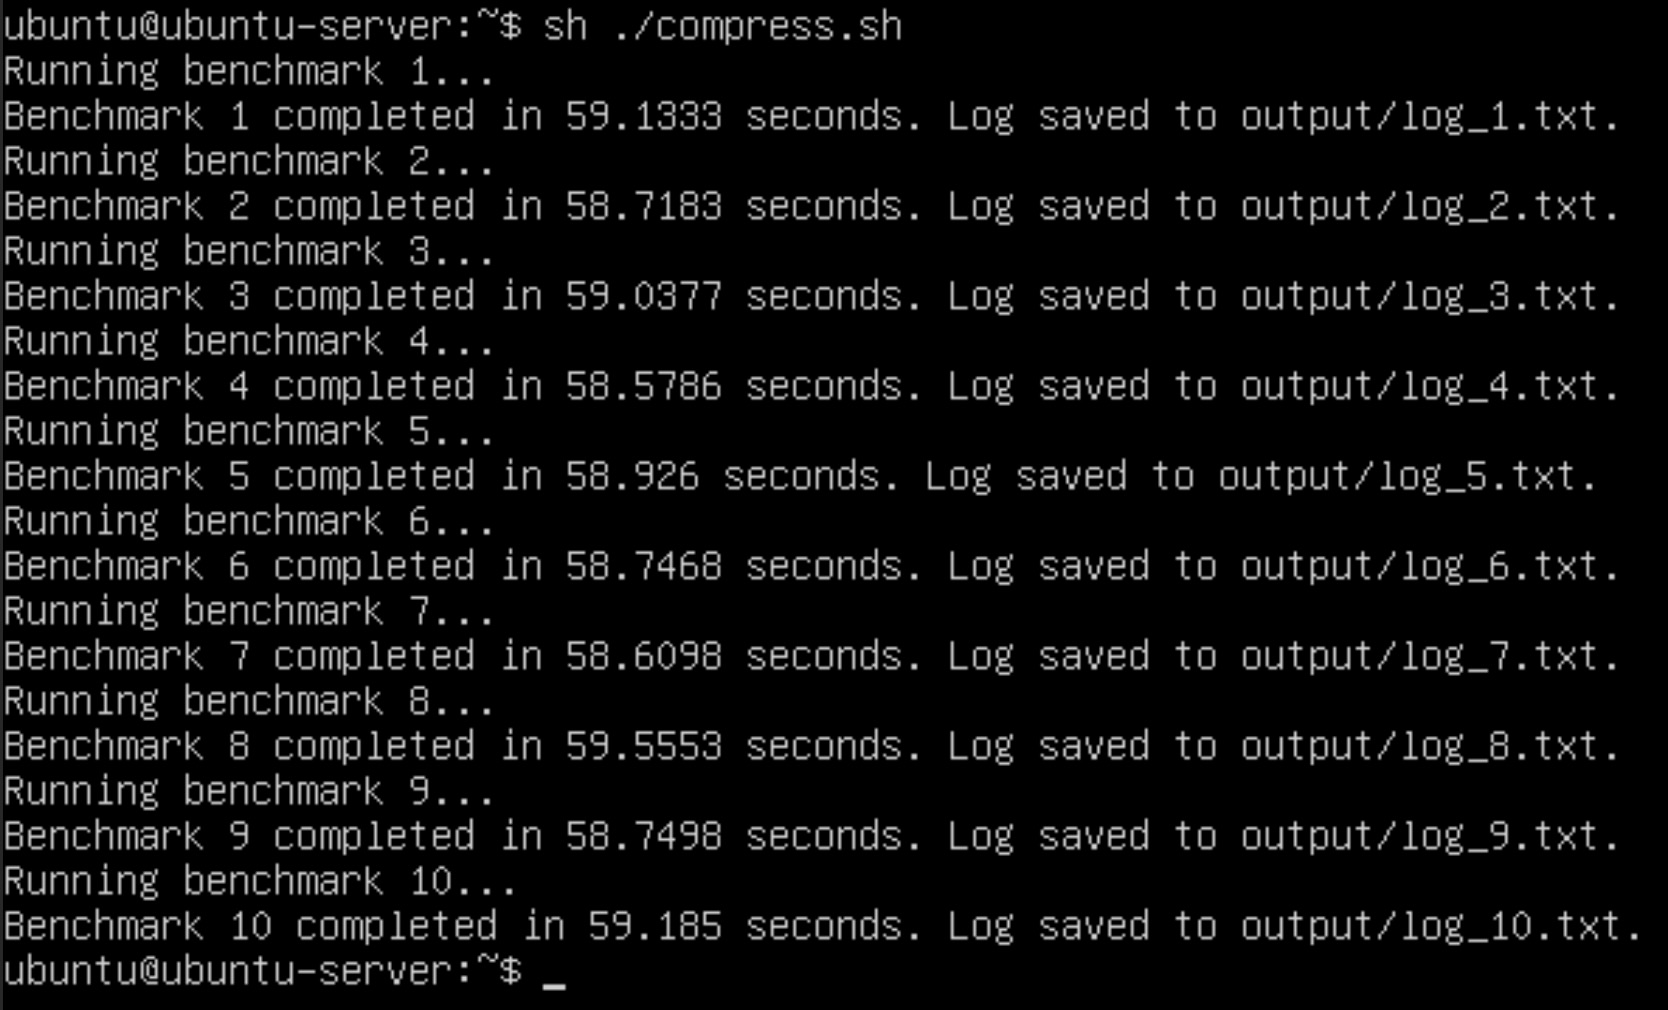
\includegraphics[width=1\textwidth]
    {assets/pics/video-compression-test/ssse3,sse4.1,sse4a.jpeg}
    \caption{Test Kompresi Video dengan Konfigurasi SSSE3 + SSE4.1 + SSE4a}
    \label{fig:video_compression_test_ssse3,sse4.1,sse4a}
\end{figure}

\begin{figure}
    \centering
    \begin{tikzpicture}
        \begin{axis}[
                xbar,
                bar width=12pt,
                xlabel={Detik},
                ytick=data,
                nodes near coords,
                nodes near coords align={horizontal},
                symbolic y coords={run 1,run 2,run 3,run 4,run 5,run 6,run 7,run 8,run 9,run 10},
                enlarge y limits=0.2,
                enlarge x limits=0.05,
                width=\textwidth,
                height=0.4\textheight,
                xmin=0,
                xmax=160
            ]
            \addplot [fill=black] coordinates {
                    (59.1333,run 1)
                    (58.7183,run 2)
                    (59.0377,run 3)
                    (58.5786,run 4)
                    (58.9260,run 5)
                    (58.7468,run 6)
                    (58.6098,run 7)
                    (59.5553,run 8)
                    (58.7498,run 9)
                    (59.1850,run 10)
                };
        \end{axis}
    \end{tikzpicture}
    \caption{Grafik Tes Kompresi Video dengan Konfigurasi SSSE3 + SSE4.1 + SSE4a}
    \label{fig:video_compression_test_ssse3,sse4.1,sse4a_graph}
\end{figure}

Program benchmark dengan kode \ref{code:kode_pengujian_kompresi_video} dijalankan pada konfigurasi SSSE3 + SSE4.1 + SSE4a. Hasil pengujian dapat dilihat pada gambar \ref{fig:video_compression_test_ssse3,sse4.1,sse4a}. Dari log yang dihasilkan saat menjalankan program benchmark, waktu yang diperlukan untuk melakukan setiap run benchmark diambil dan digunakan untuk membuat grafik seperti yang terlihat pada gambar \ref{fig:video_compression_test_ssse3,sse4.1,sse4a_graph}. Grafik tersebut menunjukkan bahwa waktu yang diperlukan untuk melakukan benchmark pada konfigurasi SSSE3 + SSE4.1 + SSE4a berkisar antara 58 detik hingga 59 detik. Rata-rata dari 10 run yang dilakukan adalah 58.9 detik.

%-----------------------------------------------------------------------------%
\subsection{Konfigurasi dengan SSSE3 + SSE4.2 + SSE4a}
%-----------------------------------------------------------------------------%
\begin{figure}
    % \centering
    % \includegraphics[width=1\textwidth]
    % {assets/pics/video-compression-test/lscpu_ssse3,sse4.2,sse4a.jpeg}
    \texttt{fpu de pse tsc msr pae mce cx8 apic sep mtrr pge mca cmov pat pse36 clflush mmx fxsr sse sse2 ht syscall nx lm rep\_good nopl cpuid extd\_apicid tsc\_known\_freq pni \textbf{ssse3} cx16 \textbf{sse4\_2} x2apic hypervisor lahf\_lm cmp\_legacy svm \textbf{sse4a} 3dnowprefetch vmmcall}
    \caption{\texttt{lscpu} Konfigurasi SSSE3 + SSE4.2 + SSE4a}
    \label{fig:lscpu_video_compression_test_ssse3,sse4.2,sse4a.jpeg}
\end{figure}

Gambar \ref{fig:lscpu_video_compression_test_ssse3,sse4.2,sse4a.jpeg} menunjukkan hasil dari perintah \texttt{lscpu} pada konfigurasi SSSE3 + SSE4.2 + SSE4a. Konfigurasi ini memiliki perubahan flag cpu \texttt{ssse3}, \texttt{sse4.2}, dan \texttt{sse4a}.

\begin{figure}
    \centering
    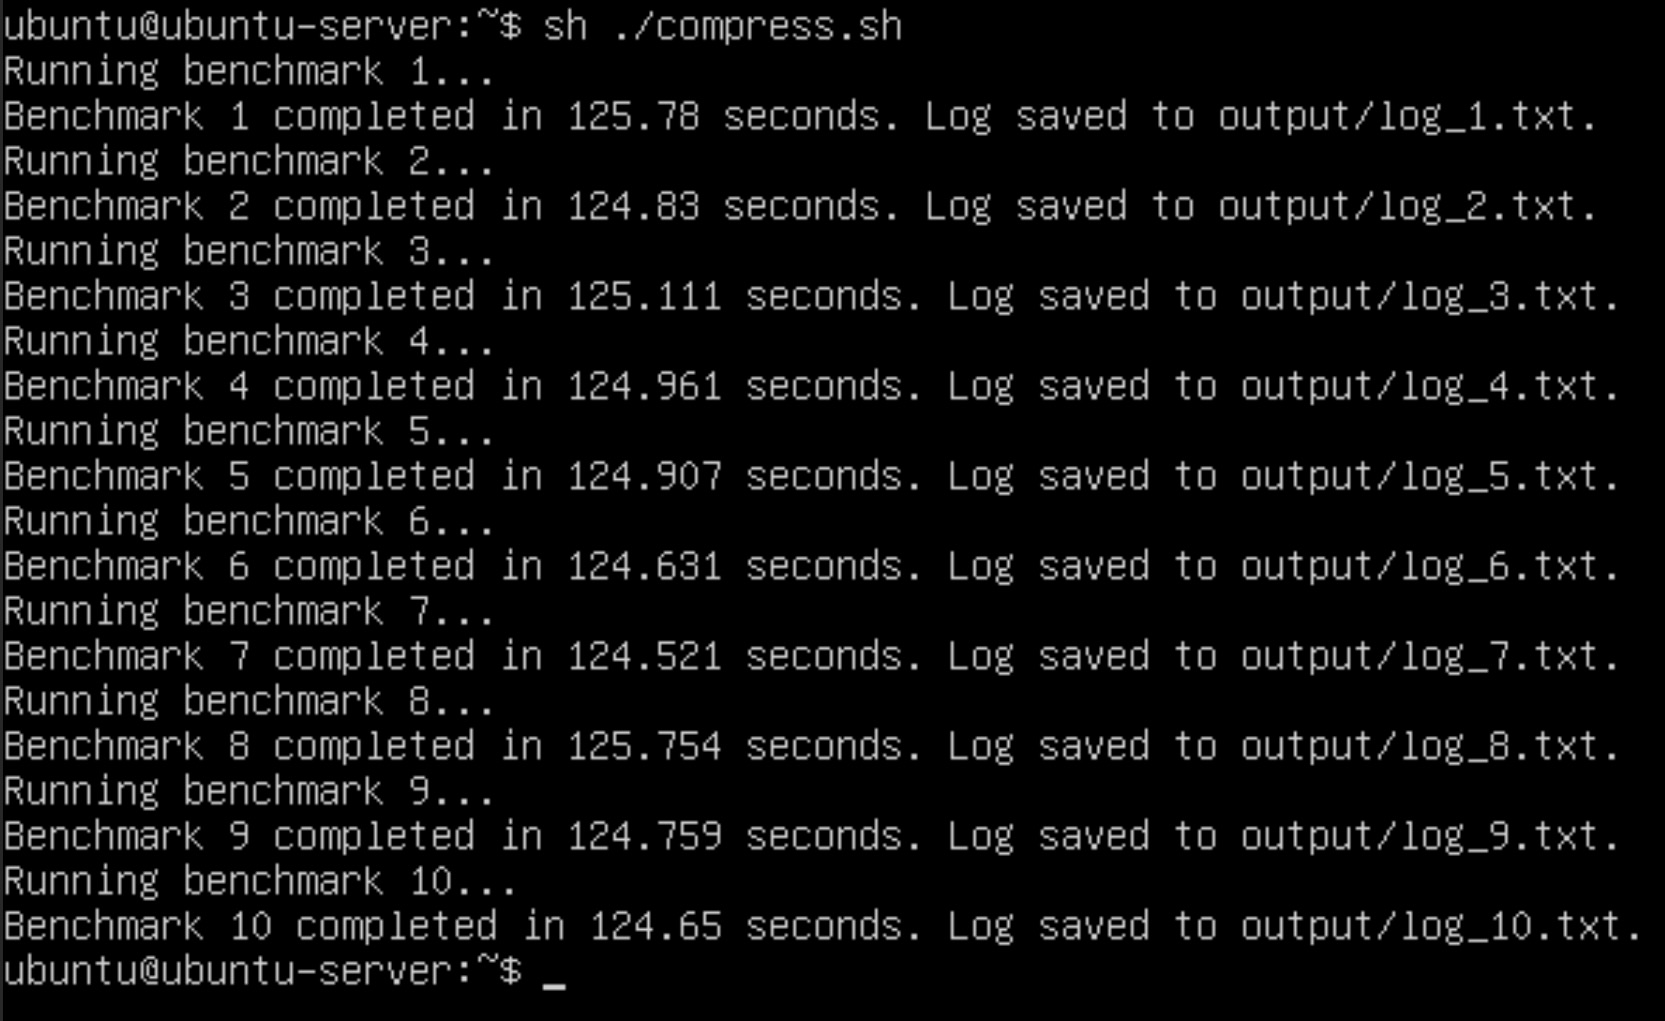
\includegraphics[width=1\textwidth]
    {assets/pics/video-compression-test/ssse3,sse4.2,sse4a.jpeg}
    \caption{Test Kompresi Video dengan Konfigurasi SSSE3 + SSE4.2 + SSE4a}
    \label{fig:video_compression_test_ssse3,sse4.2,sse4a.jpeg}
\end{figure}

\begin{figure}
    \centering
    \begin{tikzpicture}
        \begin{axis}[
                xbar,
                bar width=12pt,
                xlabel={Detik},
                ytick=data,
                nodes near coords,
                nodes near coords align={horizontal},
                symbolic y coords={run 1,run 2,run 3,run 4,run 5,run 6,run 7,run 8,run 9,run 10},
                enlarge y limits=0.2,
                enlarge x limits=0.05,
                width=\textwidth,
                height=0.4\textheight,
                xmin=0,
                xmax=160
            ]
            \addplot [fill=black] coordinates {
                    (125.780,run 1)
                    (124.830,run 2)
                    (125.111,run 3)
                    (124.961,run 4)
                    (124.907,run 5)
                    (124.631,run 6)
                    (124.521,run 7)
                    (125.754,run 8)
                    (124.759,run 9)
                    (124.650,run 10)
                };
        \end{axis}
    \end{tikzpicture}
    \caption{Grafik Tes Kompresi Video dengan Konfigurasi SSSE3 + SSE4.2 + SSE4a}
    \label{fig:video_compression_test_ssse3,sse4.2,sse4a_graph}
\end{figure}

Program benchmark dengan kode \ref{code:kode_pengujian_kompresi_video} dijalankan pada konfigurasi SSSE3 + SSE4.2 + SSE4a. Hasil pengujian dapat dilihat pada gambar \ref{fig:video_compression_test_ssse3,sse4.2,sse4a.jpeg}. Dari log yang dihasilkan saat menjalankan program benchmark, waktu yang diperlukan untuk melakukan setiap run benchmark diambil dan digunakan untuk membuat grafik seperti yang terlihat pada gambar \ref{fig:video_compression_test_ssse3,sse4.2,sse4a_graph} Grafik tersebut menunjukkan bahwa waktu yang diperlukan untuk melakukan benchmark pada konfigurasi SSSE3 + SSE4.2 + SSE4a berkisar antara 124 detik hingga 125 detik. Rata-rata dari 10 run yang dilakukan adalah 124.9 detik.
%-----------------------------------------------------------------------------%
\subsection{Konfigurasi dengan SSE4.1 + SSE4.2 + SSE4a}
%-----------------------------------------------------------------------------%
\begin{figure}
    % \centering
    % \includegraphics[width=1\textwidth]
    % {assets/pics/video-compression-test/lscpu_sse4.1,sse4.2,sse4a.jpeg}
    \texttt{fpu de pse tsc msr pae mce cx8 apic sep mtrr pge mca cmov pat pse36 clflush mmx fxsr sse sse2 ht syscall nx lm rep\_good nopl cpuid extd\_apicid tsc\_known\_freq pni cx16 \textbf{sse4\_1} \textbf{sse4\_2} x2apic hypervisor lahf\_lm cmp\_legacy svm \textbf{sse4a} 3dnowprefetch vmmcall}
    \caption{\texttt{lscpu} Konfigurasi SSE4.1 + SSE4.2 + SSE4a}
    \label{fig:lscpu_video_compression_test_sse4.1,sse4.2,sse4a.jpeg}
\end{figure}

Gambar \ref{fig:lscpu_video_compression_test_sse4.1,sse4.2,sse4a.jpeg} menunjukkan hasil dari perintah \texttt{lscpu} pada konfigurasi SSE4.1 + SSE4.2 + SSE4a. Konfigurasi ini memiliki perubahan flag cpu \texttt{sse4.1}, \texttt{sse4.2}, dan \texttt{sse4a}.

\begin{figure}
    \centering
    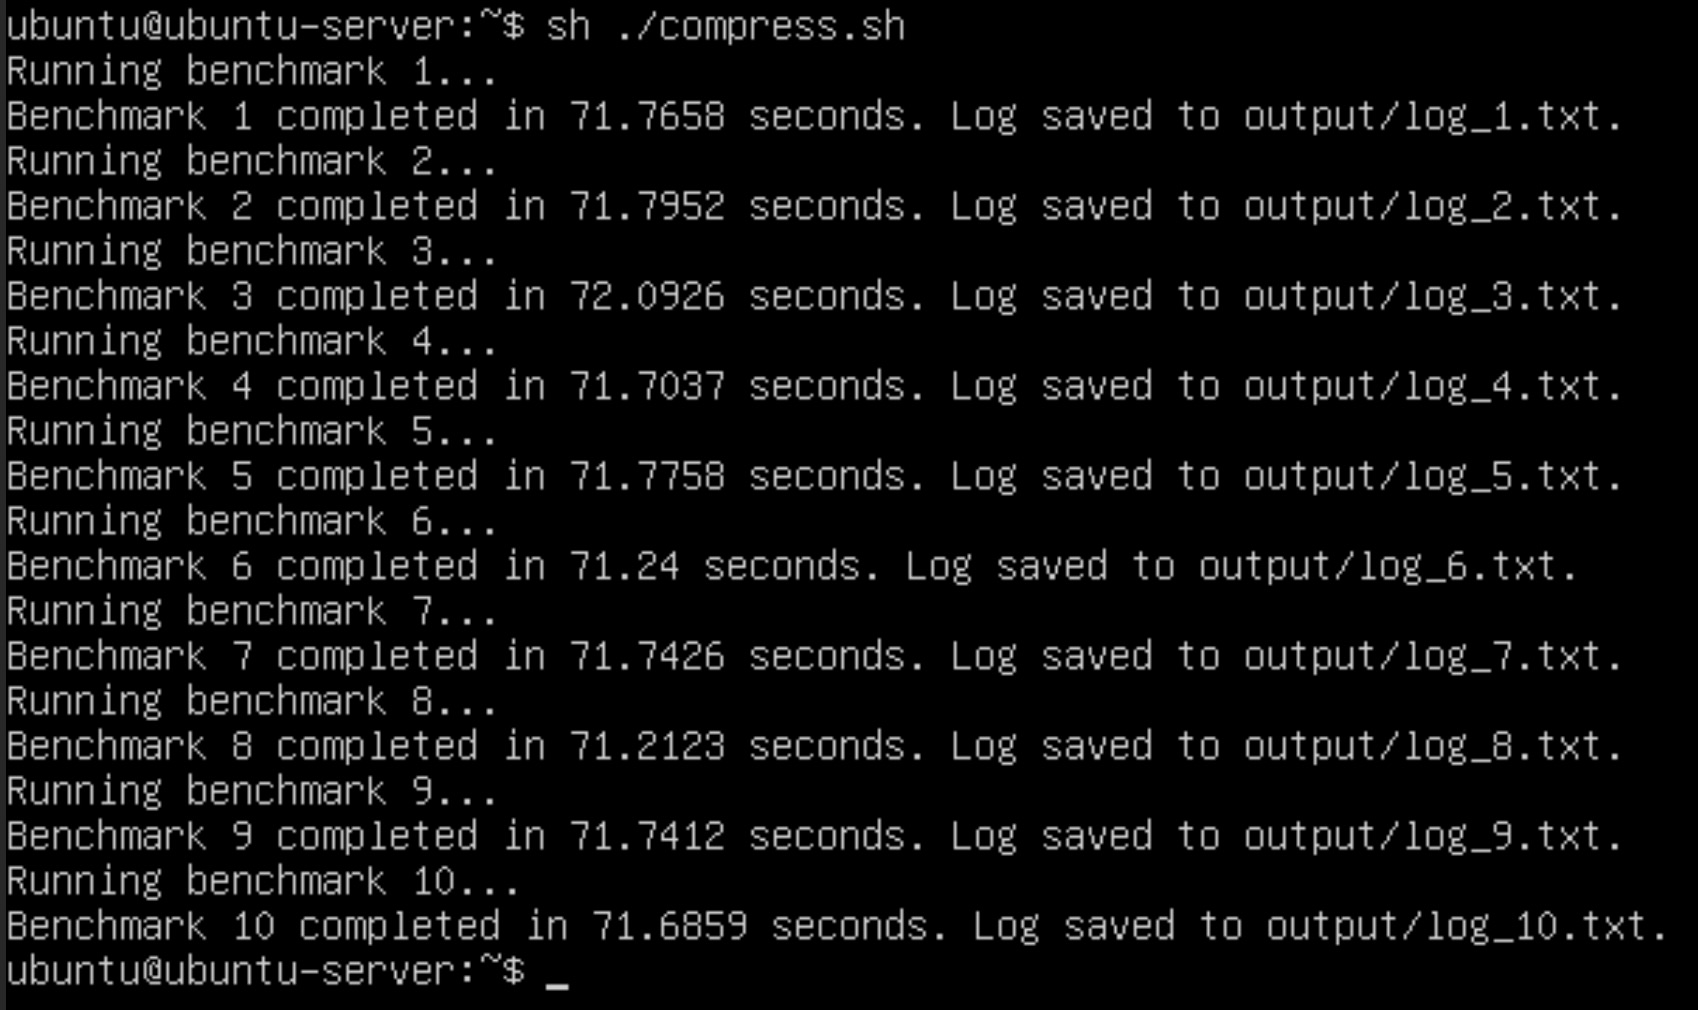
\includegraphics[width=1\textwidth]
    {assets/pics/video-compression-test/sse4.1,sse4.2,sse4a.jpeg}
    \caption{Test Kompresi Video dengan Konfigurasi SSE4.1 + SSE4.2 + SSE4a}
    \label{fig:video_compression_test_sse4.1,sse4.2,sse4a.jpeg}
\end{figure}

\begin{figure}
    \centering
    \begin{tikzpicture}
        \begin{axis}[
                xbar,
                bar width=12pt,
                xlabel={Detik},
                ytick=data,
                nodes near coords,
                nodes near coords align={horizontal},
                symbolic y coords={run 1,run 2,run 3,run 4,run 5,run 6,run 7,run 8,run 9,run 10},
                enlarge y limits=0.2,
                enlarge x limits=0.05,
                width=\textwidth,
                height=0.4\textheight,
                xmin=0,
                xmax=160
            ]
            \addplot [fill=black] coordinates {
                    (71.7658,run 1)
                    (71.7952,run 2)
                    (72.0926,run 3)
                    (71.7037,run 4)
                    (71.7758,run 5)
                    (71.2400,run 6)
                    (71.7426,run 7)
                    (71.2123,run 8)
                    (71.7412,run 9)
                    (71.6859,run 10)
                };
        \end{axis}
    \end{tikzpicture}
    \caption{Grafik Tes Kompresi Video dengan Konfigurasi SSE4.1 + SSE4.2 + SSE4a}
    \label{fig:video_compression_test_sse4.1,sse4.2,sse4a_graph}
\end{figure}

Program benchmark dengan kode \ref{code:kode_pengujian_kompresi_video} dijalankan pada konfigurasi SSE4.1 + SSE4.2 + SSE4a. Hasil pengujian dapat dilihat pada gambar \ref{fig:video_compression_test_sse4.1,sse4.2,sse4a.jpeg}. Dari log yang dihasilkan saat menjalankan program benchmark, waktu yang diperlukan untuk melakukan setiap run benchmark diambil dan digunakan untuk membuat grafik seperti yang terlihat pada gambar \ref{fig:video_compression_test_sse4.1,sse4.2,sse4a_graph}. Grafik tersebut menunjukkan bahwa waktu yang diperlukan untuk melakukan benchmark pada konfigurasi SSE4.1 + SSE4.2 + SSE4a berkisar antara 71 detik hingga 72 detik. Rata-rata dari 10 run yang dilakukan adalah 71.6 detik.

%-----------------------------------------------------------------------------%
\subsection{Konfigurasi dengan SSSE3 + SSE4.1 + SSE4.2 + SSE4a}
%-----------------------------------------------------------------------------%
\begin{figure}
    \texttt{fpu de pse tsc msr pae mce cx8 apic sep mtrr pge mca cmov pat pse36 clflush mmx fxsr sse sse2 ht syscall nx lm rep\_good nopl cpuid extd\_apicid tsc\_known\_freq pni \textbf{ssse3} cx16 \textbf{sse4\_1} \textbf{sse4\_2} x2apic hypervisor lahf\_lm cmp\_legacy svm \textbf{sse4a} 3dnowprefetch vmmcall}
    \caption{\texttt{lscpu} Konfigurasi SSSE3 + SSE4.1 + SSE4.2 + SSE4a}
    \label{fig:lscpu_video_compression_test_ssse3,sse4.1,sse4.2,sse4a.jpeg}
\end{figure}

Gambar \ref{fig:lscpu_video_compression_test_ssse3,sse4.1,sse4a} menunjukkan hasil dari perintah \texttt{lscpu} pada konfigurasi SSSE3 + SSE4.1 + SSE4.2 + SSE4a. Konfigurasi ini memiliki perubahan flag cpu \texttt{ssse3}, \texttt{sse4.1}, \texttt{sse4.2}, dan \texttt{sse4a}.

\begin{figure}
    \centering
    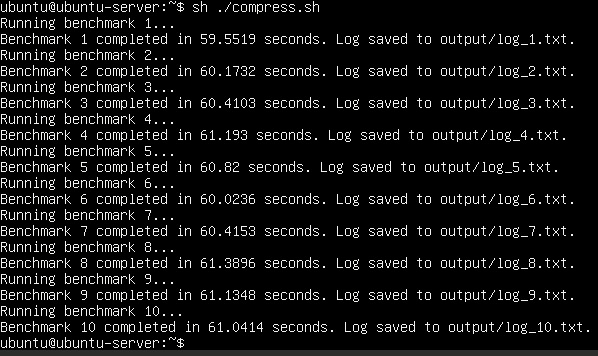
\includegraphics[width=1\textwidth]
    {assets/pics/video-compression-test/ssse3,sse4.1,sse4.2,sse4a.jpeg}
    \caption{Test Kompresi Video dengan Konfigurasi SSSE3 + SSE4.1 + SSE4.2 + SSE4a}
    \label{fig:video_compression_test_ssse3,sse4.1,sse4.2,sse4a.jpeg}
\end{figure}

\begin{figure}
    \centering
    \begin{tikzpicture}
        \begin{axis}[
                xbar,
                bar width=12pt,
                xlabel={Detik},
                ytick=data,
                nodes near coords,
                nodes near coords align={horizontal},
                symbolic y coords={run 1,run 2,run 3,run 4,run 5,run 6,run 7,run 8,run 9,run 10},
                enlarge y limits=0.2,
                enlarge x limits=0.05,
                width=\textwidth,
                height=0.4\textheight,
                xmin=0,
                xmax=160
            ]
            \addplot [fill=black] coordinates {
                    (59.5519,run 1)
                    (60.1732,run 2)
                    (60.4103,run 3)
                    (61.1930,run 4)
                    (60.8200,run 5)
                    (60.0236,run 6)
                    (60.4153,run 7)
                    (61.3896,run 8)
                    (61.1348,run 9)
                    (61.0414,run 10)
                };
        \end{axis}
    \end{tikzpicture}
    \caption{Grafik Tes Kompresi Video dengan Konfigurasi SSSE3 + SSE4.1 + SSE4.2 + SSE4a}
    \label{fig:video_compression_test_ssse3,sse4.1,sse4.2,sse4a_graph}
\end{figure}

Program benchmark dengan kode \ref{code:kode_pengujian_kompresi_video} dijalankan pada konfigurasi SSSE3 + SSE4.1 + SSE4.2 + SSE4a. Hasil pengujian dapat dilihat pada gambar \ref{fig:video_compression_test_ssse3,sse4.1,sse4.2,sse4a.jpeg}. Dari log yang dihasilkan saat menjalankan program benchmark, waktu yang diperlukan untuk melakukan setiap run benchmark diambil dan digunakan untuk membuat grafik seperti yang terlihat pada gambar \ref{fig:video_compression_test_ssse3,sse4.1,sse4.2,sse4a_graph} Grafik tersebut menunjukkan bahwa waktu yang diperlukan untuk melakukan benchmark pada konfigurasi SSSE3 + SSE4.1 + SSE4.2 + SSE4a berkisar antara 59 detik hingga 61 detik. Rata-rata dari 10 run yang dilakukan adalah 60.1 detik.

%-----------------------------------------------------------------------------%
\subsection{Analisis Pengujian Tuning Hypervisor KVM dengan Kompresi Video}
%-----------------------------------------------------------------------------%
% \begin{figure}
%     \centering
%     \begin{tikzpicture}
%         \begin{axis}[
%                 xbar,
%                 bar width=12pt,
%                 xlabel={Detik},
%                 ytick=data,
%                 nodes near coords,
%                 nodes near coords align={horizontal},
%                 symbolic y coords={4.1.1,4.1.2,4.1.3,4.1.4,4.1.5,4.1.6,4.1.7,4.1.8,4.1.9,4.1.10,4.1.11,4.1.12,4.1.13,4.1.14,4.1.15,4.1.16},
%                 enlarge y limits=0.1,
%                 enlarge x limits=0.05,
%                 width=\textwidth,
%                 height=0.5\textheight,
%                 xmin=0,
%                 xmax=160
%             ]
%             \addplot [fill=black] coordinates {
%                     (141.5,4.1.1)
%                     (126.5,4.1.2)
%                     (73.2,4.1.3)
%                     (142.7,4.1.4)
%                     (140.8,4.1.5)
%                     (58.2,4.1.6)
%                     (123.5,4.1.7)
%                     (124.4,4.1.8)
%                     (70.34,4.1.9)
%                     (69.9,4.1.10)
%                     (139.1,4.1.11)
%                     (59.1,4.1.12)
%                     (58.9,4.1.13)
%                     (124.9,4.1.14)
%                     (71.6,4.1.15)
%                     (60.1,4.1.16)
%                 };
%         \end{axis}
%     \end{tikzpicture}
%     \caption{Grafik Rata-Rata Waktu Tes Kompresi Video}
%     \label{fig:video_compression_test_graph}
% \end{figure}

% Grafik \ref{fig:video_compression_test_graph} menunjukkan rata-rata waktu yang diperlukan untuk melakukan benchmark pada setiap konfigurasi yang diuji. Dari grafik tersebut, dapat dilihat bahwa konfigurasi yang memiliki waktu tercepat adalah konfigurasi SSSE3 + SSE4.1 dengan rata-rata waktu 58.2 detik.

\begin{figure}
    \centering
    \begin{tikzpicture}
        \begin{axis}[
                xbar,
                bar width=12pt,
                xlabel={\f{Speedup}},
                ytick=data,
                nodes near coords,
                nodes near coords align={horizontal},
                symbolic y coords={4.1.1,4.1.2,4.1.3,4.1.4,4.1.5,4.1.6,4.1.7,4.1.8,4.1.9,4.1.10,4.1.11,4.1.12,4.1.13,4.1.14,4.1.15,4.1.16},
                enlarge y limits=0.1,
                enlarge x limits=0.05,
                width=\textwidth,
                height=0.5\textheight,
                xmin=0,
                xmax=2.6
            ]
            \addplot [fill=black] coordinates {
                    (1.0000,4.1.1)
                    (1.1180,4.1.2)
                    (1.9330,4.1.3)
                    (0.9910,4.1.4)
                    (1.0049,4.1.5)
                    (2.4310,4.1.6)
                    (1.1450,4.1.7)
                    (1.1370,4.1.8)
                    (2.0110,4.1.9)
                    (2.0240,4.1.10)
                    (1.0170,4.1.11)
                    (2.3940,4.1.12)
                    (2.4020,4.1.13)
                    (1.1329,4.1.14)
                    (1.9760,4.1.15)
                    (2.3540,4.1.16)
                };
        \end{axis}
    \end{tikzpicture}
    \caption{Grafik \f{speedup} Tes Kompresi Video}
    \label{fig:video_compression_test_graph}
\end{figure}

Grafik \ref{fig:video_compression_test_graph} menunjukkan \f{speedup} dari setiap konfigurasi yang diuji. Dari grafik tersebut, dapat dilihat bahwa konfigurasi yang memiliki \f{speedup} tertinggi adalah konfigurasi SSSE3 + SSE4.1 denga nilai \f{speedup} 2.431, dengan rata-rata waktu untuk melakukan kompresi selama 58.2 detik.

%-----------------------------------------------------------------------------%
\section{Hasil Pengujian Tuning Hypervisor KVM dengan Validasi Integritas Data}
%-----------------------------------------------------------------------------%
Pada bagian ini akan dijelaskan hasil pengujian tuning hypervisor KVM dengan validasi integritas data dengan menggunakan program benchmark kode \ref{code:kode_pengujian_validasi_integritas_data}.

%-----------------------------------------------------------------------------%
\subsection{Konfigurasi Default}
%-----------------------------------------------------------------------------%
\begin{figure}
    % \centering
    % \includegraphics[width=1\textwidth]
    % {assets/pics/video-compression-test/lscpu_ssse3,sse4.1,sse4a.jpeg}
    \texttt{fpu de pse tsc msr pae mce cx8 apic sep mtrr pge mca cmov pat pse36 clflush mmx fxsr sse sse2 ht syscall nx lm rep\_good nopl cpuid extd\_apicid tsc\_known\_freq pni cx16 x2apic hypervisor lahf\_lm cmp\_legacy svm 3dnowprefetch vmmcall}
    \caption{\texttt{lscpu} Konfigurasi Default}
    \label{fig:lscpu_file_integrity_test_default}
\end{figure}

Gambar \ref{fig:lscpu_file_integrity_test_default} menunjukkan hasil dari perintah \texttt{lscpu} pada konfigurasi default. Konfigurasi ini tidak memiliki perubahan flag cpu.

\begin{figure}
    \centering
    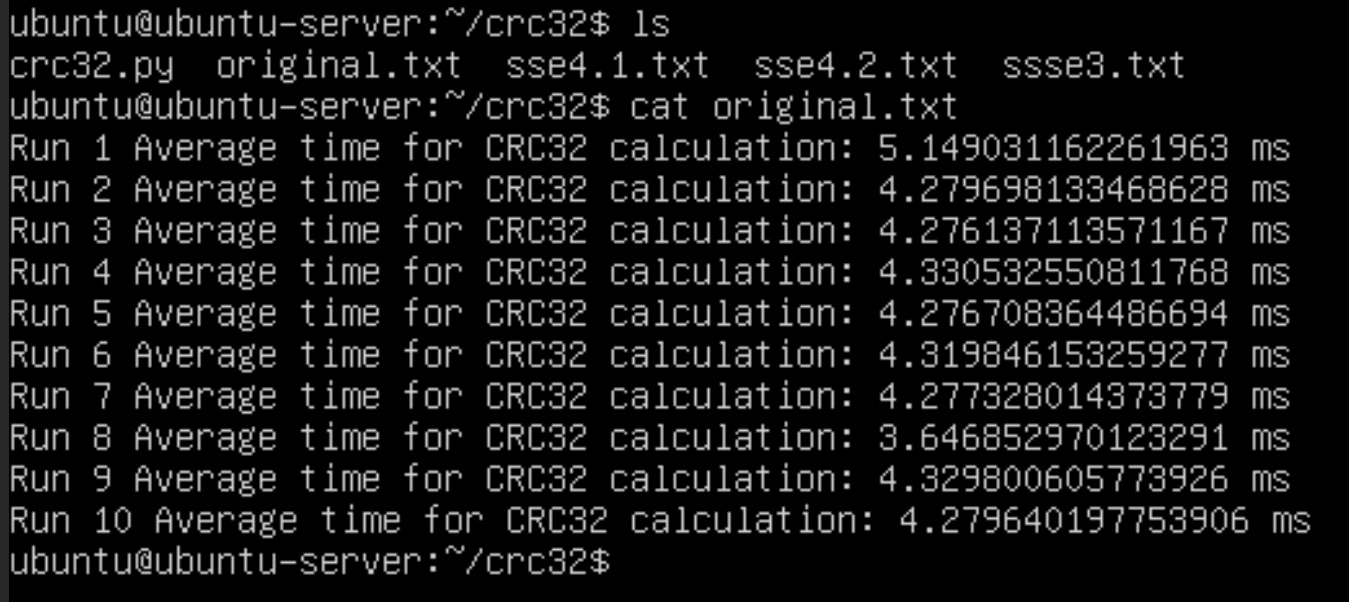
\includegraphics[width=1\textwidth]
    {assets/pics/crc-test/original.jpeg}
    \caption{Test Validasi Integritas Data Dengan Konfigurasi Default}
    \label{fig:file_integrity_test_default}
\end{figure}

\begin{figure}
    \centering
    \begin{tikzpicture}
        \begin{axis}[
                xbar,
                bar width=12pt,
                xlabel={Milisecond},
                ytick=data,
                nodes near coords,
                nodes near coords align={horizontal},
                symbolic y coords={run 1,run 2,run 3,run 4,run 5,run 6,run 7,run 8,run 9,run 10},
                enlarge y limits=0.2,
                enlarge x limits=0.05,
                width=\textwidth,
                height=0.4\textheight,
                xmin=0,
                xmax=5.5
            ]
            \addplot [fill=black] coordinates {
                    (5.149,run 1)
                    (4.279,run 2)
                    (4.276,run 3)
                    (4.330,run 4)
                    (4.276,run 5)
                    (4.319,run 6)
                    (4.277,run 7)
                    (3.646,run 8)
                    (4.329,run 9)
                    (4.279,run 10)
                };
        \end{axis}
    \end{tikzpicture}
    \caption{Grafik Tes Validasi Integritas Data Dengan Konfigurasi Default}
    \label{fig:file_integrity_test_default_graph}
\end{figure}

Program benchmark dengan kode \ref{code:kode_pengujian_validasi_integritas_data} dijalankan pada konfigurasi default. Hasil pengujian dapat dilihat pada gambar \ref{fig:file_integrity_test_default}. Dari log yang dihasilkan saat menjalankan program benchmark, waktu yang diperlukan untuk melakukan setiap run benchmark diambil dan digunakan untuk membuat grafik seperti yang terlihat pada gambar \ref{fig:file_integrity_test_default_graph}. Grafik tersebut menunjukkan bahwa waktu yang diperlukan untuk melakukan benchmark pada konfigurasi default berkisar antara 3.6 ms hingga 5.1 ms. Rata-rata dari 10 run yang dilakukan adalah 4.3 ms.

%-----------------------------------------------------------------------------%
\subsection{Konfigurasi dengan SSE4.2}
%-----------------------------------------------------------------------------%
\begin{figure}
    % \centering
    % \includegraphics[width=1\textwidth]
    % {assets/pics/video-compression-test/lscpu_ssse3,sse4.1,sse4a.jpeg}
    \texttt{fpu de pse tsc msr pae mce cx8 apic sep mtrr pge mca cmov pat pse36 clflush mmx fxsr sse sse2 ht syscall nx lm rep\_good nopl cpuid extd\_apicid tsc\_known\_freq pni cx16 \textbf{sse4\_2} x2apic hypervisor lahf\_lm cmp\_legacy svm 3dnowprefetch vmmcall}
    \caption{\texttt{lscpu} Konfigurasi SSE4.2}
    \label{fig:lscpu_file_integrity_test_sse4.2}
\end{figure}

Gambar \ref{fig:lscpu_file_integrity_test_sse4.2} menunjukkan hasil dari perintah \texttt{lscpu} pada konfigurasi SSE4.2. Konfigurasi ini memiliki perubahan flag cpu \texttt{sse4.2}.

\begin{figure}
    \centering
    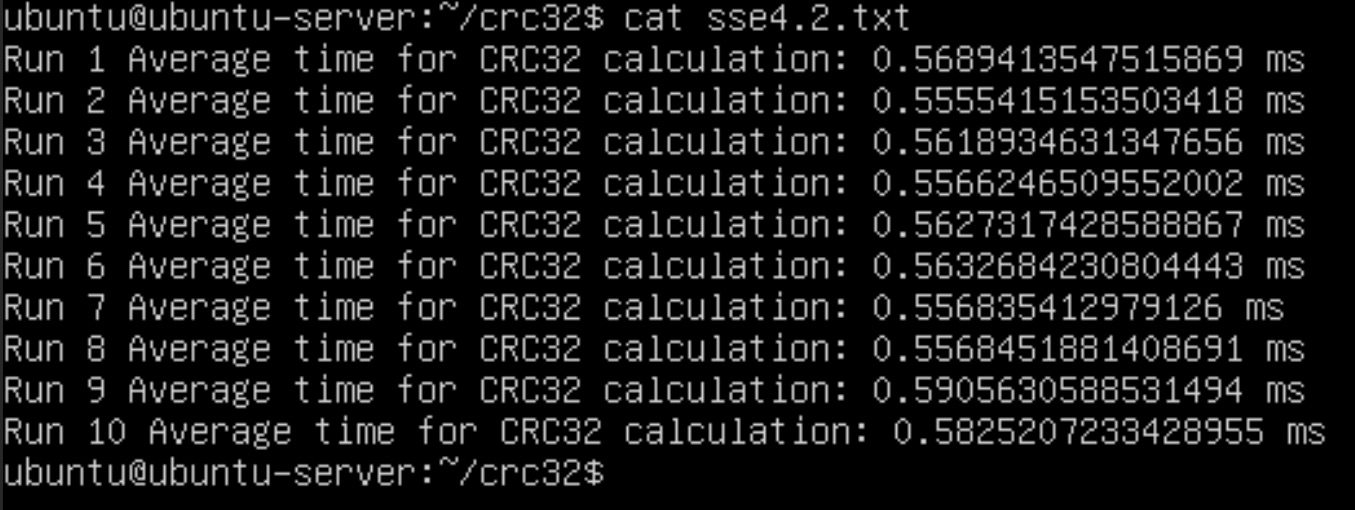
\includegraphics[width=1\textwidth]
    {assets/pics/crc-test/sse4.2.jpeg}
    \caption{Test Validasi Integritas Data Dengan Konfigurasi SSE4.2}
    \label{fig:file_integrity_test_sse4.2}
\end{figure}

\begin{figure}
    \centering
    \begin{tikzpicture}
        \begin{axis}[
                xbar,
                bar width=12pt,
                xlabel={Milisecond},
                ytick=data,
                nodes near coords,
                nodes near coords align={horizontal},
                symbolic y coords={run 1,run 2,run 3,run 4,run 5,run 6,run 7,run 8,run 9,run 10},
                enlarge y limits=0.2,
                enlarge x limits=0.05,
                width=\textwidth,
                height=0.4\textheight,
                xmin=0,
                xmax=5.5
            ]
            \addplot [fill=black] coordinates {
                    (0.568,run 1)
                    (0.555,run 2)
                    (0.561,run 3)
                    (0.556,run 4)
                    (0.562,run 5)
                    (0.563,run 6)
                    (0.556,run 7)
                    (0.556,run 8)
                    (0.590,run 9)
                    (0.582,run 10)
                };
        \end{axis}
    \end{tikzpicture}
    \caption{Grafik Tes Validasi Integritas Data Dengan Konfigurasi SSE4.2}
    \label{fig:file_integrity_test_sse4.2_graph}
\end{figure}

Program benchmark dengan kode \ref{code:kode_pengujian_validasi_integritas_data} dijalankan pada konfigurasi SSE4.2. Hasil pengujian dapat dilihat pada gambar \ref{fig:file_integrity_test_sse4.2}. Dari log yang dihasilkan saat menjalankan program benchmark, waktu yang diperlukan untuk melakukan setiap run benchmark diambil dan digunakan untuk membuat grafik seperti yang terlihat pada gambar \ref{fig:file_integrity_test_sse4.2_graph}. Grafik tersebut menunjukkan bahwa waktu yang diperlukan untuk melakukan benchmark pada konfigurasi SSE4.2 berkisar antara 0.55 ms hingga 0.59 ms. Rata-rata dari 10 run yang dilakukan adalah 0.56 ms.

%-----------------------------------------------------------------------------%
\subsection{Analisis Pengujian Tuning Hypervisor KVM dengan Validasi Integritas Data}
%-----------------------------------------------------------------------------%

% \begin{figure}
%     \centering
%     \begin{tikzpicture}
%         \begin{axis}[
%                 xbar,
%                 bar width=12pt,
%                 xlabel={Milisecond},
%                 ytick=data,
%                 nodes near coords,
%                 nodes near coords align={horizontal},
%                 symbolic y coords={4.2.1,4.2.2},
%                 enlarge y limits=0.2,
%                 enlarge x limits=0.05,
%                 width=\textwidth,
%                 height=0.2\textheight,
%                 xmin=0,
%                 xmax=5.5
%             ]
%             \addplot [fill=black] coordinates {
%                     (4.3,4.2.1)
%                     (0.56,4.2.2)
%                 };
%         \end{axis}
%     \end{tikzpicture}
%     \caption{Grafik Rata-Rata Waktu Tes Validasi Integritas Data}
%     \label{fig:file_integrity_test_graph}
% \end{figure}

% Grafik \ref{fig:file_integrity_test_graph} menunjukkan rata-rata waktu yang diperlukan untuk melakukan benchmark pada setiap konfigurasi yang diuji. Dari grafik tersebut, dapat dilihat bahwa konfigurasi yang memiliki waktu tercepat adalah konfigurasi SSE4.2 dengan rata-rata waktu 0.56 ms.

\begin{figure}
    \centering
    \begin{tikzpicture}
        \begin{axis}[
                xbar,
                bar width=12pt,
                xlabel={\f{Speedup}},
                ytick=data,
                nodes near coords,
                nodes near coords align={horizontal},
                symbolic y coords={4.2.1,4.2.2},
                enlarge y limits=0.2,
                enlarge x limits=0.05,
                width=\textwidth,
                height=0.2\textheight,
                xmin=0,
                xmax=8
            ]
            \addplot [fill=black] coordinates {
                    (1.000,4.2.1)
                    (7.678,4.2.2)
                };
        \end{axis}
    \end{tikzpicture}
    \caption{Grafik \f{speedup} Tes Validasi Integritas Data}
    \label{fig:file_integrity_test_graph}
\end{figure}

Grafik \ref{fig:file_integrity_test_graph} menunjukkan \f{speedup} dari setiap konfigurasi yang diuji. Dari grafik tersebut, dapat dilihat bahwa konfigurasi yang memiliki \f{speedup} tertinggi adalah konfigurasi SSE4.2 dengan nilai \f{speedup} 7.678, dengan rata-rata waktu untuk melakukan validasi integritas data selama 0.56 ms.

%-----------------------------------------------------------------------------%
\section{Hasil Pengujian Tuning Hypervisor KVM dengan Enkripsi AES}
%-----------------------------------------------------------------------------%
Pada bagian ini akan dijelaskan hasil pengujian tuning hypervisor KVM dengan enkripsi AES dengan menggunakan program benchmark kode \ref{code:pengujian_enkripsi_aes}.

%-----------------------------------------------------------------------------%
\subsection{Konfigurasi Default}
%-----------------------------------------------------------------------------%
\begin{figure}
    % \centering
    % \includegraphics[width=1\textwidth]
    % {assets/pics/video-compression-test/lscpu_ssse3,sse4.1,sse4a.jpeg}
    \texttt{fpu de pse tsc msr pae mce cx8 apic sep mtrr pge mca cmov pat pse36 clflush mmx fxsr sse sse2 ht syscall nx lm rep\_good nopl cpuid extd\_apicid tsc\_known\_freq pni cx16 x2apic hypervisor lahf\_lm cmp\_legacy svm 3dnowprefetch vmmcall}
    \caption{\texttt{lscpu} Konfigurasi Default}
    \label{fig:lscpu_aes_test_default}
\end{figure}

Gambar \ref{fig:lscpu_aes_test_default} menunjukkan hasil dari perintah \texttt{lscpu} pada konfigurasi default. Konfigurasi ini tidak memiliki perubahan flag cpu.

\begin{figure}
    \centering
    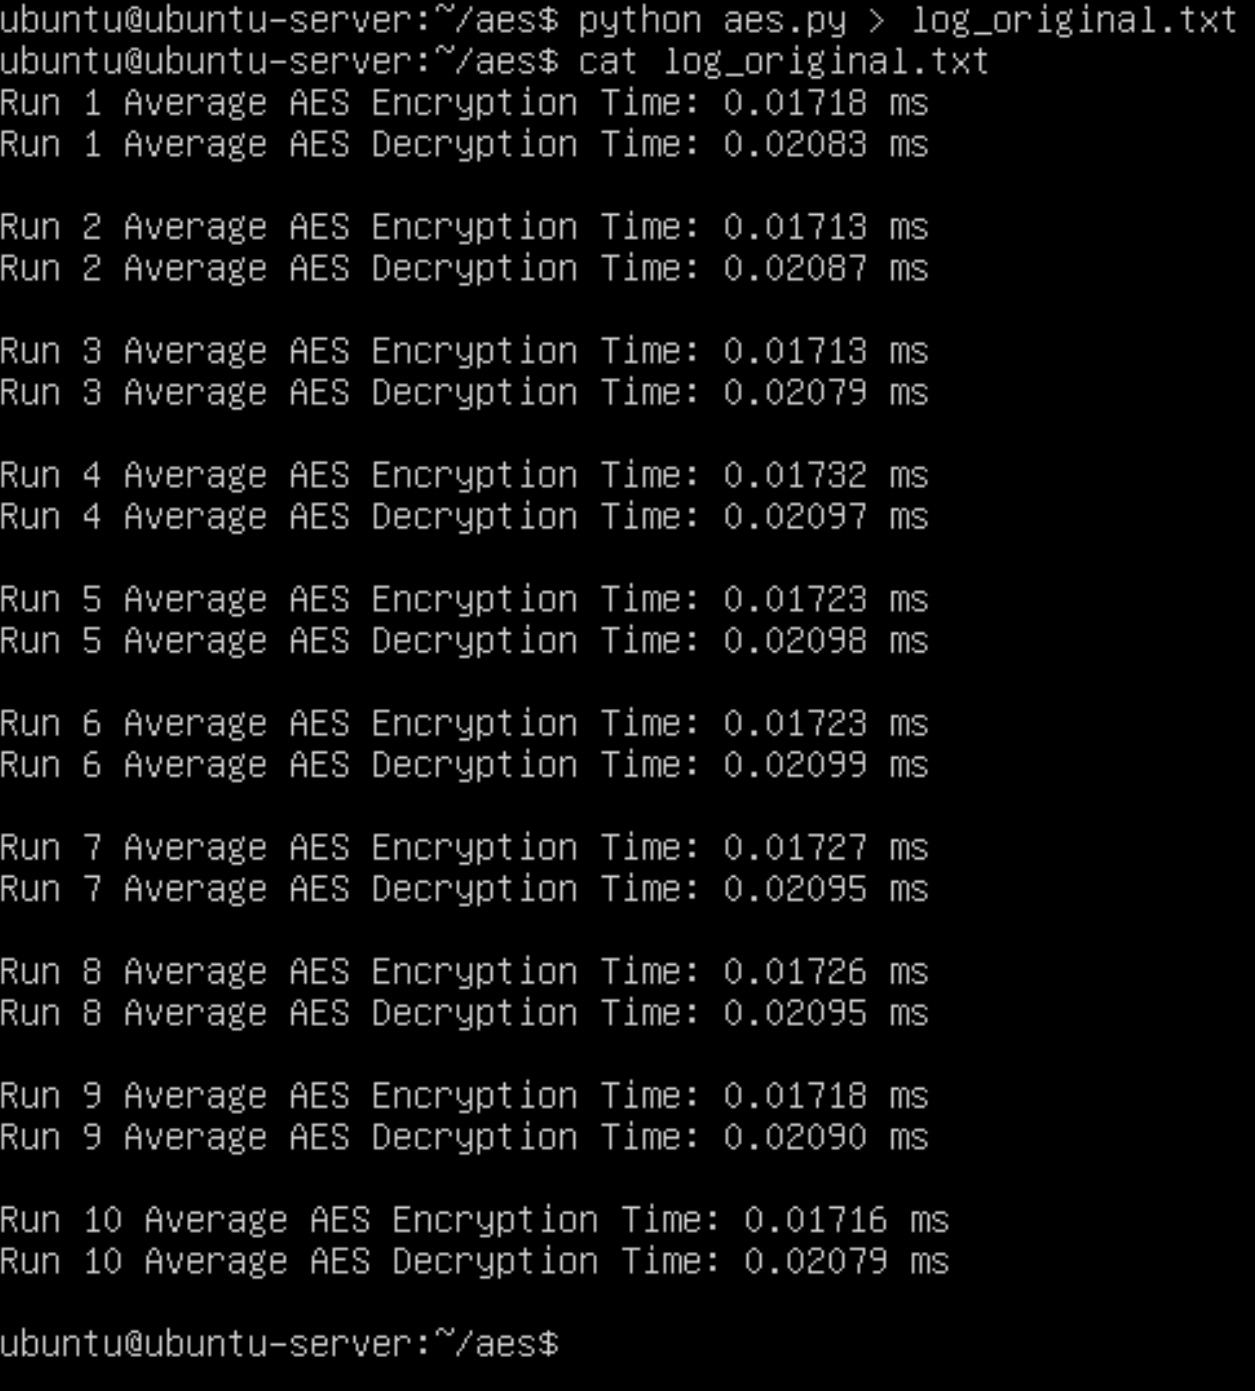
\includegraphics[width=1\textwidth]
    {assets/pics/aes-test/original.jpeg}
    \caption{Test Enkripsi AES Dengan Konfigurasi Default}
    \label{fig:aes_test_default}
\end{figure}

\begin{figure}
    \centering
    \begin{tikzpicture}
        \begin{axis}[
                xbar,
                bar width=12pt,
                xlabel={Microsecond},
                ytick=data,
                nodes near coords,
                nodes near coords align={horizontal},
                symbolic y coords={run 1,run 2,run 3,run 4,run 5,run 6,run 7,run 8,run 9,run 10},
                enlarge y limits=0.2,
                enlarge x limits=0.05,
                width=\textwidth,
                height=0.4\textheight,
                xmin=0,
                xmax=23
            ]
            \addplot [fill=black] coordinates {
                    (17.180,run 1)
                    (17.130,run 2)
                    (17.130,run 3)
                    (17.320,run 4)
                    (17.230,run 5)
                    (17.230,run 6)
                    (17.270,run 7)
                    (17.260,run 8)
                    (17.180,run 9)
                    (17.160,run 10)
                };
        \end{axis}
    \end{tikzpicture}
    \caption{Grafik Tes Enkripsi AES Dengan Konfigurasi Default}
    \label{fig:aes_encryption_test_default_graph}
\end{figure}

\begin{figure}
    \centering
    \begin{tikzpicture}
        \begin{axis}[
                xbar,
                bar width=12pt,
                xlabel={Microsecond},
                ytick=data,
                nodes near coords,
                nodes near coords align={horizontal},
                symbolic y coords={run 1,run 2,run 3,run 4,run 5,run 6,run 7,run 8,run 9,run 10},
                enlarge y limits=0.2,
                enlarge x limits=0.05,
                width=\textwidth,
                height=0.4\textheight,
                xmin=0,
                xmax=23
            ]
            \addplot [fill=black] coordinates {
                    (20.830,run 1)
                    (20.870,run 2)
                    (20.790,run 3)
                    (20.970,run 4)
                    (20.980,run 5)
                    (20.990,run 6)
                    (20.950,run 7)
                    (20.950,run 8)
                    (20.900,run 9)
                    (20.790,run 10)
                };
        \end{axis}
    \end{tikzpicture}
    \caption{Grafik Tes Dekripsi AES Dengan Konfigurasi Default}
    \label{fig:aes_decryption_test_default_graph}
\end{figure}

Program benchmark dengan kode \ref{code:pengujian_enkripsi_aes} dijalankan pada konfigurasi default. Hasil pengujian dapat dilihat pada gambar \ref{fig:aes_test_default}. Dari log yang dihasilkan saat menjalankan program benchmark, waktu yang diperlukan untuk melakukan setiap run benchmark diambil dan digunakan untuk membuat grafik seperti yang terlihat pada gambar \ref{fig:aes_encryption_test_default_graph} dan \ref{fig:aes_decryption_test_default_graph}. Grafik tersebut menunjukkan bahwa waktu yang diperlukan untuk melakukan benchmark pada konfigurasi default berkisar untuk melakukan enkripsi berkisar antara 17 $\mu$s hingga 17.3 $\mu$s dan untuk melakukan dekripsi berkisar antara 20.7 $\mu$s hingga 21 $\mu$s. Rata-rata dari 10 run yang dilakukan adalah 17.2 $\mu$sms untuk enkripsi dan 20.9 $\mu$s untuk dekripsi.

%-----------------------------------------------------------------------------%
\subsection{Konfigurasi dengan AES}
%-----------------------------------------------------------------------------%
\begin{figure}
    % \centering
    % \includegraphics[width=1\textwidth]
    % {assets/pics/video-compression-test/lscpu_ssse3,sse4.1,sse4a.jpeg}
    \texttt{fpu de pse tsc msr pae mce cx8 apic sep mtrr pge mca cmov pat pse36 clflush mmx fxsr sse sse2 ht syscall nx lm rep\_good nopl cpuid extd\_apicid tsc\_known\_freq pni cx16 x2apic \textbf{aes} hypervisor lahf\_lm cmp\_legacy svm 3dnowprefetch vmmcall}
    \caption{\texttt{lscpu} Konfigurasi AES}
    \label{fig:lscpu_aes_test_aes}
\end{figure}

Gambar \ref{fig:lscpu_aes_test_aes} menunjukkan hasil dari perintah \texttt{lscpu} pada konfigurasi AES. Konfigurasi ini memiliki perubahan flag cpu \texttt{aes}.

\begin{figure}
    \centering
    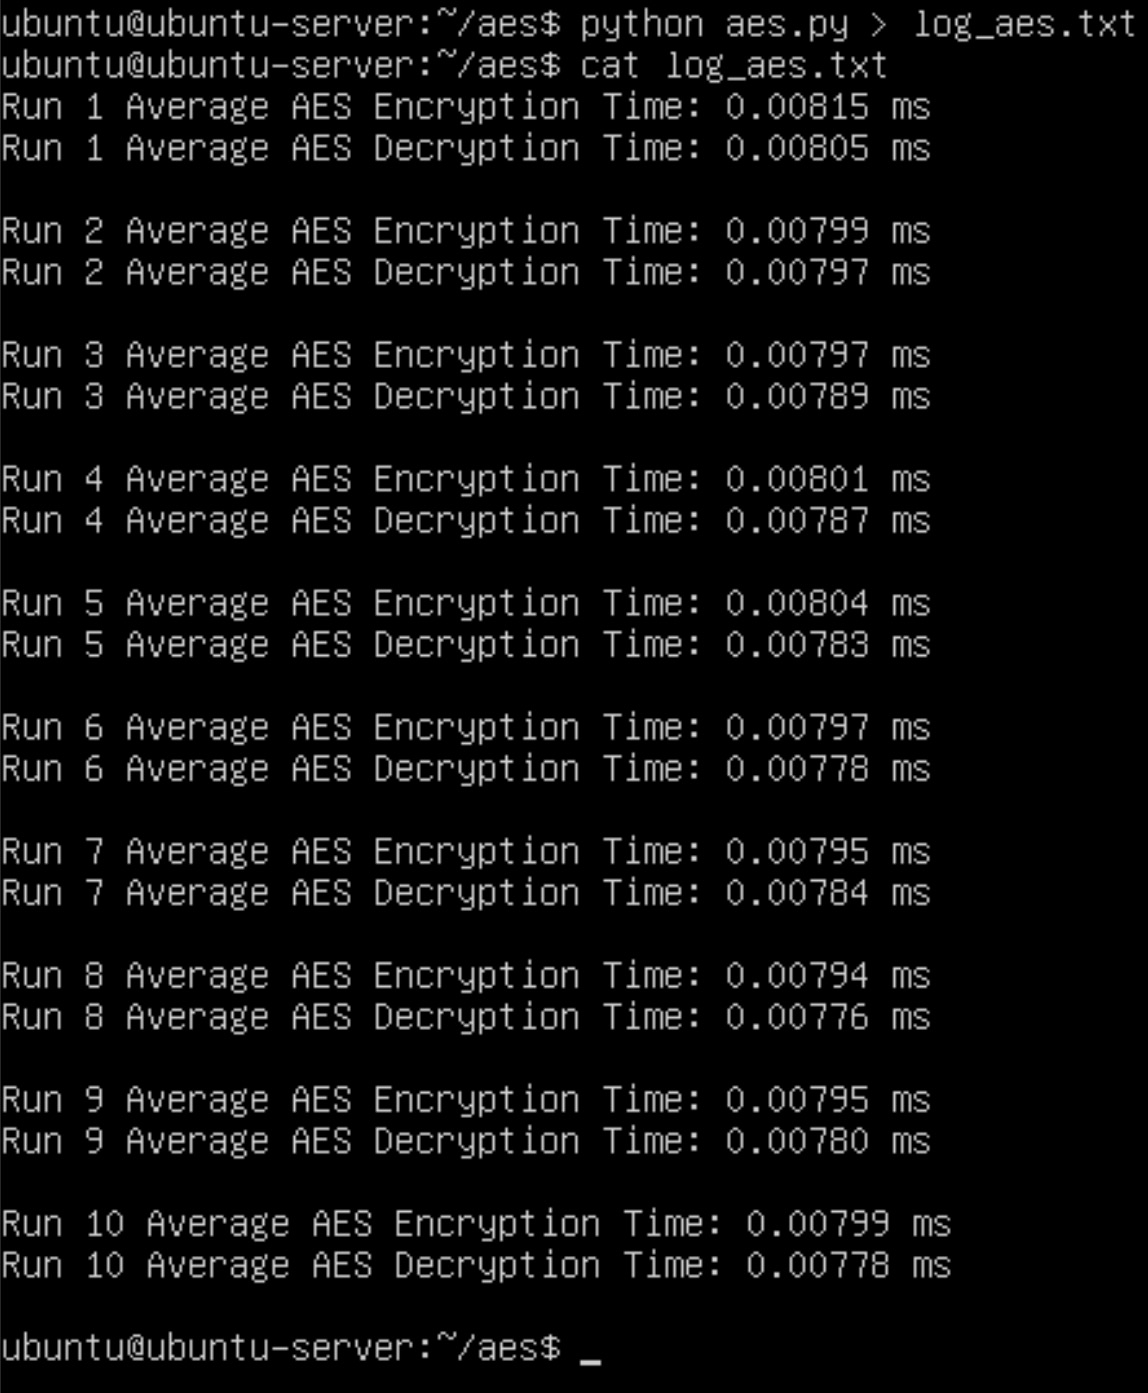
\includegraphics[width=1\textwidth]
    {assets/pics/aes-test/aes.jpeg}
    \caption{Test Enkripsi AES Dengan Konfigurasi AES}
    \label{fig:aes_test_aes}
\end{figure}

\begin{figure}
    \centering
    \begin{tikzpicture}
        \begin{axis}[
                xbar,
                bar width=12pt,
                xlabel={Microsecond},
                ytick=data,
                nodes near coords,
                nodes near coords align={horizontal},
                symbolic y coords={run 1,run 2,run 3,run 4,run 5,run 6,run 7,run 8,run 9,run 10},
                enlarge y limits=0.2,
                enlarge x limits=0.05,
                width=\textwidth,
                height=0.4\textheight,
                xmin=0,
                xmax=23
            ]
            \addplot [fill=black] coordinates {
                    (8.150,run 1)
                    (7.990,run 2)
                    (7.970,run 3)
                    (8.010,run 4)
                    (8.040,run 5)
                    (7.970,run 6)
                    (7.950,run 7)
                    (7.940,run 8)
                    (7.950,run 9)
                    (7.990,run 10)
                };
        \end{axis}
    \end{tikzpicture}
    \caption{Grafik Tes Enkripsi AES Dengan Konfigurasi AES}
    \label{fig:aes_encryption_test_aes_graph}
\end{figure}

\begin{figure}
    \centering
    \begin{tikzpicture}
        \begin{axis}[
                xbar,
                bar width=12pt,
                xlabel={Microsecond},
                ytick=data,
                nodes near coords,
                nodes near coords align={horizontal},
                symbolic y coords={run 1,run 2,run 3,run 4,run 5,run 6,run 7,run 8,run 9,run 10},
                enlarge y limits=0.2,
                enlarge x limits=0.05,
                width=\textwidth,
                height=0.4\textheight,
                xmin=0,
                xmax=23
            ]
            \addplot [fill=black] coordinates {
                    (8.050,run 1)
                    (7.970,run 2)
                    (7.890,run 3)
                    (7.870,run 4)
                    (7.830,run 5)
                    (7.780,run 6)
                    (7.840,run 7)
                    (7.760,run 8)
                    (7.800,run 9)
                    (7.780,run 10)
                };
        \end{axis}
    \end{tikzpicture}
    \caption{Grafik Tes Dekripsi AES Dengan Konfigurasi AES}
    \label{fig:aes_decryption_test_aes_graph}
\end{figure}

Program benchmark dengan kode \ref{code:pengujian_enkripsi_aes} dijalankan pada konfigurasi AES. Hasil pengujian dapat dilihat pada gambar \ref{fig:aes_test_aes}. Dari log yang dihasilkan saat menjalankan program benchmark, waktu yang diperlukan untuk melakukan setiap run benchmark diambil dan digunakan untuk membuat grafik seperti yang terlihat pada gambar \ref{fig:aes_encryption_test_aes_graph} dan \ref{fig:aes_decryption_test_aes_graph}. Grafik tersebut menunjukkan bahwa waktu yang diperlukan untuk melakukan benchmark pada konfigurasi AES berkisar untuk melakukan enkripsi berkisar antara 7.8 $\mu$s hingga 8.15 $\mu$s dan untuk melakukan dekripsi berkisar antara 7.76 $\mu$s hingga 8.05 $\mu$s. Rata-rata dari 10 run yang dilakukan adalah 7.9 $\mu$s untuk enkripsi dan 7.8 $\mu$s untuk dekripsi.

%-----------------------------------------------------------------------------%
\subsection{Analisis Pengujian Tuning Hypervisor KVM dengan Enkripsi AES}
%-----------------------------------------------------------------------------%

% \begin{figure}
%     \centering
%     \begin{tikzpicture}
%         \begin{axis}[
%                 xbar,
%                 bar width=12pt,
%                 xlabel={Microsecond},
%                 ytick=data,
%                 nodes near coords,
%                 nodes near coords align={horizontal},
%                 symbolic y coords={4.3.1,4.3.2},
%                 enlarge y limits=0.2,
%                 enlarge x limits=0.05,
%                 width=\textwidth,
%                 height=0.2\textheight,
%                 xmin=0,
%                 xmax=23
%             ]
%             \addplot [fill=black] coordinates {
%                     (17.2,4.3.1)
%                     (7.9,4.3.2)
%                 };
%         \end{axis}
%     \end{tikzpicture}
%     \caption{Grafik Rata-Rata Waktu Tes Enkripsi AES}
%     \label{fig:aes_encrypt_test_graph}
% \end{figure}

% \begin{figure}
%     \centering
%     \begin{tikzpicture}
%         \begin{axis}[
%                 xbar,
%                 bar width=12pt,
%                 xlabel={Microsecond},
%                 ytick=data,
%                 nodes near coords,
%                 nodes near coords align={horizontal},
%                 symbolic y coords={4.3.1,4.3.2},
%                 enlarge y limits=0.2,
%                 enlarge x limits=0.05,
%                 width=\textwidth,
%                 height=0.2\textheight,
%                 xmin=0,
%                 xmax=23
%             ]
%             \addplot [fill=black] coordinates {
%                     (20.9,4.3.1)
%                     (7.8,4.3.2)
%                 };
%         \end{axis}
%     \end{tikzpicture}
%     \caption{Grafik Rata-Rata Waktu Tes Dekripsi AES}
%     \label{fig:aes_decrypt_test_graph}
% \end{figure}

% Grafik \ref{fig:aes_encrypt_test_graph} dan \ref{fig:aes_decrypt_test_graph} menunjukkan rata-rata waktu yang diperlukan untuk melakukan benchmark pada setiap konfigurasi yang diuji. Dari grafik tersebut, dapat dilihat bahwa konfigurasi yang memiliki waktu tercepat adalah konfigurasi AES dengan rata-rata waktu 7.9 $\mu$s untuk enkripsi dan 7.8 $\mu$s untuk dekripsi.

\begin{figure}
    \centering
    \begin{tikzpicture}
        \begin{axis}[
                xbar,
                bar width=12pt,
                xlabel={Microsecond},
                ytick=data,
                nodes near coords,
                nodes near coords align={horizontal},
                symbolic y coords={4.3.1,4.3.2},
                enlarge y limits=0.2,
                enlarge x limits=0.05,
                width=\textwidth,
                height=0.2\textheight,
                xmin=0,
                xmax=3
            ]
            \addplot [fill=black] coordinates {
                    (1.00,4.3.1)
                    (2.17,4.3.2)
                };
        \end{axis}
    \end{tikzpicture}
    \caption{Grafik Rata-Rata Waktu Tes Enkripsi AES}
    \label{fig:aes_encrypt_test_graph}
\end{figure}

\begin{figure}
    \centering
    \begin{tikzpicture}
        \begin{axis}[
                xbar,
                bar width=12pt,
                xlabel={Microsecond},
                ytick=data,
                nodes near coords,
                nodes near coords align={horizontal},
                symbolic y coords={4.3.1,4.3.2},
                enlarge y limits=0.2,
                enlarge x limits=0.05,
                width=\textwidth,
                height=0.2\textheight,
                xmin=0,
                xmax=3
            ]
            \addplot [fill=black] coordinates {
                    (1.000,4.3.1)
                    (2.679,4.3.2)
                };
        \end{axis}
    \end{tikzpicture}
    \caption{Grafik Rata-Rata Waktu Tes Dekripsi AES}
    \label{fig:aes_decrypt_test_graph}
\end{figure}

Grafik \ref{fig:aes_encrypt_test_graph} dan \ref{fig:aes_decrypt_test_graph} menunjukkan \f{speedup} dari setiap konfigurasi yang diuji. Dari grafik tersebut, dapat dilihat bahwa konfigurasi yang memiliki \f{speedup} tertinggi adalah konfigurasi AES dengan nilai \f{speedup} 2.17 untuk enkripsi dan 2.679 untuk dekripsi. Dengan masing masing rata-rata waktu untuk melakukan enkripsi dan dekripsi adalah 7.9 $\mu$s dan 7.8 $\mu$s.


\iffalse
    %-----------------------------------------------------------------------------%
    %\chapter{\babEmpat}
    %-----------------------------------------------------------------------------%
    \todo{tambahkan kata-kata pengantar bab 1 disini}

    %-----------------------------------------------------------------------------%
    \section{thesis.tex}
    %-----------------------------------------------------------------------------%
    Berkas ini berisi seluruh berkas Latex yang dibaca, jadi bisa dikatakan sebagai
    berkas utama. Dari berkas ini kita dapat mengatur bab apa saja yang ingin
    kita tampilkan dalam dokumen.


    %-----------------------------------------------------------------------------%
    \section{laporan\_setting.tex}
    %-----------------------------------------------------------------------------%
    Berkas ini berguna untuk mempermudah pembuatan beberapa template standar.
    Anda diminta untuk menuliskan judul laporan, nama, npm, dan hal-hal lain yang
    dibutuhkan untuk pembuatan template.


    %-----------------------------------------------------------------------------%
    \section{istilah.tex}
    %-----------------------------------------------------------------------------%
    Berkas istilah digunakan untuk mencatat istilah-istilah yang digunakan.
    Fungsinya hanya untuk memudahkan penulisan.
    Pada beberapa kasus, ada kata-kata yang harus selalu muncul dengan tercetak
    miring atau tercetak tebal.
    Dengan menjadikan kata-kata tersebut sebagai sebuah perintah \latex~tentu akan
    mempercepat dan mempermudah pengerjaan laporan.


    %-----------------------------------------------------------------------------%
    \section{hype.indonesia.tex}
    %-----------------------------------------------------------------------------%
    Berkas ini berisi cara pemenggalan beberapa kata dalam bahasa Indonesia.
    \latex~memiliki algoritma untuk memenggal kata-kata sendiri, namun untuk
    beberapa kasus algoritma ini memenggal dengan cara yang salah.
    Untuk memperbaiki pemenggalan yang salah inilah cara pemenggalan yang benar
    ditulis dalam berkas hype.indonesia.tex.


    %-----------------------------------------------------------------------------%
    \section{pustaka.tex}
    %-----------------------------------------------------------------------------%
    Berkas pustaka.tex berisi seluruh daftar referensi yang digunakan dalam
    laporan.
    Anda bisa membuat model daftar referensi lain dengan menggunakan bibtex.
    Untuk mempelajari bibtex lebih lanjut, silahkan buka
    \url{http://www.bibtex.org/Format}.
    Untuk merujuk pada salah satu referensi yang ada, gunakan perintah \bslash
    cite, e.g. \bslash cite\{lankton2008introduction\} yang akan akan memunculkan
    \cite{lankton2008introduction}


    %-----------------------------------------------------------------------------%
    \section{bab[1 - 6].tex}
    %-----------------------------------------------------------------------------%
    Berkas ini berisi isi laporan yang Anda tulis.
    Setiap nama berkas e.g. bab1.tex merepresentasikan bab dimana tulisan tersebut
    akan muncul.
    Sebagai contoh, kode dimana tulisan ini dibaut berada dalam berkas dengan nama
    bab4.tex.
    Ada enam buah berkas yang telah disiapkan untuk mengakomodir enam bab dari
    laporan Anda, diluar bab kesimpulan dan saran.
    Jika Anda tidak membutuhkan sebanyak itu, silahkan hapus kode dalam berkas
    thesis.tex yang memasukan berkas \latex~yang tidak dibutuhkan;  contohnya
    perintah \bslash include\{bab6.tex\} merupakan kode untuk memasukan berkas
    bab6.tex kedalam laporan.

    %-----------------------------------------------------------------------------%
    \section{Penulisan \textit{code} atau \textit{pseudocode} program}
    %-----------------------------------------------------------------------------%

    \subsection{\textit{Inline}}

    Dengan perintah \verb|\verb|: \verb|System.out.println("Hello, World");| \\
    Dengan perintah \textit{custom} \verb|\code|: \code{System.out.println("Hello, World"); }
    Dengan perintah \verb|\mintinline|: \mintinline{java}{System.out.println("Hello, World"); }

    \subsection{\textit{Multiline}}

    Dengan perintah \verb|verbatim|:

    \begin{verbatim}	
public class HelloWorld {
    public static void main(String[] args) {
        // Prints "Hello, World" to the terminal window.
        System.out.println("Hello, World");
    }
}
\end{verbatim}

    Dengan perintah \verb|minted|: Kode \ref{code:hw:minted}
    \begin{listing}[H]
        \begin{minted}{python}
def binary_accuracy(y_true, y_pred):
    return K.mean(K.equal(y_true, K.round(y_pred)), axis=-1)


def categorical_accuracy(y_true, y_pred):
    return K.cast(K.equal(K.argmax(y_true, axis=-1),
                          K.argmax(y_pred, axis=-1)),
                  K.floatx())


def sparse_categorical_accuracy(y_true, y_pred):
    # reshape in case it's in shape (num_samples, 1) instead of (num_samples,)
    if K.ndim(y_true) == K.ndim(y_pred):
        y_true = K.squeeze(y_true, -1)
    # convert dense predictions to labels
    y_pred_labels = K.argmax(y_pred, axis=-1)
    y_pred_labels = K.cast(y_pred_labels, K.floatx())
    return K.cast(K.equal(y_true, y_pred_labels), K.floatx())


def top_k_categorical_accuracy(y_true, y_pred, k=5):
    return K.mean(K.in_top_k(y_pred, K.argmax(y_true, axis=-1), k), axis=-1)


def sparse_top_k_categorical_accuracy(y_true, y_pred, k=5):
    # If the shape of y_true is (num_samples, 1), flatten to (num_samples,)
    return K.mean(K.in_top_k(y_pred, K.cast(K.flatten(y_true), 'int32'), k),
                  axis=-1)
    \end{minted}
        \caption{An excerpt from keras: \url{https://github.com/keras-team/keras/blob/master/keras/metrics.py}}
        \label{code:hw:minted}
    \end{listing}

    Konfigurasi tampilan bisa dilakukan di \verb|uithesis.sty| dengan referensi dokumentasi di \url{https://github.com/gpoore/minted/blob/master/source/minted.pdf}

\fi